\documentclass{ucbthesis}
%\usepackage{biblatex}
\usepackage[backend=bibtex]{biblatex}
%\usepackage[style=numeric]{biblatex}
%\addbibresource{mybib.bib}
\DeclareNameAlias{default}{last-first}
\usepackage{graphicx}
\usepackage{amsmath}
\usepackage{amsthm}
\usepackage{amsfonts}
\usepackage{mathtools}
\usepackage{float}
\usepackage{algorithm2e}
\DeclarePairedDelimiter{\ceil}{\lceil}{\rceil}
\setlength{\parindent}{0em}
\setlength{\parskip}{1em}
% Double spacing, if you want it.
% \def\dsp{\def\baselinestretch{2.0}\large\normalsize}
% \dsp

% If the Grad. Division insists that the first paragraph of a section
% be indented (like the others), then include this line:
% \usepackage{indentfirst}

\newtheorem{theorem}{Theorem}[section]
\newtheorem{corollary}{Corollary}[theorem]
\newtheorem{prop}{Proposition}
\newtheorem{lemma}[theorem]{Lemma}
\theoremstyle{definition}
\newtheorem{definition}{Definition}[section]

 
\theoremstyle{remark}
\newtheorem*{remark}{Remark}

\bibliography{references}

\hyphenation{mar-gin-al-ia}

\begin{document}

% Declarations for Front Matter

\title{Inference on Graphs: From Probability Methods to Deep Neural Networks}
\author{Xiang Li}
\degreesemester{Spring}
\degreeyear{2017}
\degree{Doctor of Philosophy}
\chair{David Aldous}
\othermembers{Joan Bruna, Lauren Williams}

\numberofmembers{3}

\field{Statistics}
\campus{Berkeley}

% For a masters thesis, uncomment (remove the % at the beginning of)
% the following line.  This affects the title and approval pages,
% which by default calls this a "dissertation", not a "thesis".

%\itsamasters

% The title page generated by LaTeX is now acceptable for handing in.
% (This was not always the case).

\maketitle
\approvalpage
\copyrightpage

% (This is included by thesis.tex; you do not latex it by itself.)

\begin{abstract}

% The text of the abstract goes here.  If you need to use a \section
% command you will need to use \section*, \subsection*, etc. so that
% you don't get any numbering.  You probably won't be using any of
% these commands in the abstract anyway.

Graphs are a rich and fundamental object of study, of interest from both theoretical and applied points of view. This thesis is in two parts and gives a treatment of graphs from two differing points of view, with the goal of doing inference on graphs.  The first is a mathematical approach.  We create a formal framework to investigate the quality of inference on graphs given partial observations.  The proofs we give apply to all graphs without assumptions.  In the second part of this thesis, we take on the problem of clustering with the aid of deep neural networks and apply it to the problem of community detection with results that are competitive with the state of the art even at the information theoretic threshold of recovery of cluster assignments in the stochastic blockmodel. 
\end{abstract}


\begin{frontmatter}

\begin{dedication}
\null\vfil
\begin{center}
To my parents. \\\vspace{12pt}

\end{center}
\vfil\null
\end{dedication}

\tableofcontents
\clearpage
\listoffigures
\clearpage


\begin{acknowledgements}
%David has provided a supportive and free environment for me to do a explore my interests.  From when I first approached him when I was still a student in the Logic department to do a .  It was an honour to be a part of the academic environment you have created, .  You 

%I also want to thank Balazs Szegedy.  Though the research of this thesis departs from our previous work in graph limits, the joy of doing mathematics that he shared with me I have held as a standard .  Sharing with .  My dearest memories in budapest
%His vision of math, from a bird eye view, approaching novel fields with the eye of an algebraist was fresh, e
%I also want to thank Joan Bruna, 

%My parents, whom I have dedicated this thesis, .  From them 

\end{acknowledgements}

\end{frontmatter}

\pagestyle{headings}

\chapter{Introduction}

Graphs, also known as networks in applied fields, are rich objects that enjoy study by mathematicians, physicists, computer scientists and social scientists.  Graph structure is fundamental and its applications are many and varied, including social networks, collaborative filtering, epidemiology, protein interactions, and image segmentation, to name just a few.  Even the theoretical underpinnings of much of the analysis tools in these disciplines are rooted in graph theory; for instance  graphical models in machine learning and clustering as a general tool for simplifying data in both theory and application.  

The mathematical treatment of graphs has been approached from many directions, from discrete mathematics and combinatorics, to analysis and probability. Randomness is oftentimes used as a tool for investigation as well a generator of interesting objects of study.  Of note is the probabilistic method and random graphs, starting from the work of Paul Erd\H{o}s.  The modern theory of Markov Chains is not to be left out given its intimate relationship with graph theory, and it will also make an appearance in this thesis. The theory of Graphons, a modern development of the past 2 decades concerns a particularly natural completion of the discrete graph space, thus allowing the theory of these discrete objects to benefit from the rich array of tools in analysis and topology.  It goes without saying that graphs have proved rich objects of study for mathematicians.  

On the other hand, applied fields have borrowed the tools and theorems proven in mathematics to inspire algorithms. A exciting young field with many such applications is the field of deep neural networks.  Deep neural networks have been extremely successful in many supervised domains, among them object detection in computer vision and machine translation are examples of applications with near human level performance or super human level performance.  This has been a demonstrated success of optimization via gradient descent like methods to gather statistical features of the large training sets.  Training sets that have become readily available to us in the last couple of years, along with the much more powerful level of computing power compared to when neural networks were first introduced more than 40 years ago.  


This thesis is in two parts.  In the first part, we create a framework for studying the quality of inferences from a partially observed graph.  Given no assumptions on the underlying``true'' graph, we are interested in rigorously understanding how to quantify a functional on the observed graph that best approximates the functional of interest on the true graph. In part two, we make inferences on graphs from an empirical point of view.  Focusing on the problem of clustering, we design a deep neural network that has within its expressive closure the ability to approximate a rich family of algorithms, and a much more expressive reach beyond that.  We test the architecture and its performance on the stochastic blockmodel as well as real data sets with community labels.  We show that our graph neural network performs competitively in these settings with no parameter assumptions as well as with less computational steps. This work is only scratching the surface of the ability of these architectures and exciting extensions are discussed.

%We give a probability model to the observed graph to rigorously study the framework. 
\part{A Probabilistic Model for Imperfectly Observed Graphs}


\chapter{The Framework}
 Two broad themes in the analysis of graphs emerge in how the theory is both related to and inspired by applications.  Let's dive in.  

\section{Analysis of Probability Models}

One topic naturally emerging from a mathematical treatment involves the analysis of probability models on graphs.  These models are usually inspired by a particular property of real world networks, and provide a more simple, contained setting in which we can test hypotheses on how such properties affect more complicated behaviour.  For instance, the small worlds network is an example of a probabilistic generative model that exhibits degree distributions similar to social networks, and so one justification for studying these graphs is that it would reveal insights into real networks. Given such a network, one would then try to quantify some random process on the graph (for instance, a random walk: what can we say about its long term dynamics as a random walk explores the graph, or how easy is it to cluster nodes so that flow is mostly trapped within clusters?).  Another way to go about it is to analyze how the family of graphs in a particular model exhibits different graph-theoretical measures.  For instance, natural ones that are motivated from applications include clustering statistics (triangle density, clique statistics, degree distributions...etc).  

In abstracted terms, the investigations above concern some graph G (stochastically or deterministically specified) and some functional $\Gamma(G)$, where oftentimes we are estimating and getting a hold of the behaviour of moments of $\Gamma(G)$ depending on parameters defining $G$.  So for example in the case of $G$ is the stochastic block model (defined in Part II), $\Gamma$ can be the edge density.  


\section{Algorithmic Efficiency/Computational Complexity}
This approach falls within the empirical regime, where algorithms take in a graph $G$ and outputs $\Gamma(G)$.  Different algorithms are compared for their performance on benchmarked data (real $G$) or well known graphs and various classical algorithms.  Examples of works in this regime include Jaewon et al.'s study of the quality of community labels in a bunch of data sets as well as the performance of clustering algorithms on them in \cite{JureJaewon_baseline_quality}, and Lu and Zhou's link prediction survey in\cite{link}.

\section{The Model}

Given the two aforementioned treatments of network analysis, we place our project in between the two paradigms.  We model the process of observing a true graph $G$ via another graph $G'$.  The theoretical question then is to understand how $\Gamma(G')$ relates to $\Gamma(G)$.  


Consider the basic structure of a social network, we have the individuals modeled as nodes of a graph and relationships between individuals modelled as edges.  In the real world, relationships are not homogeneous and a simple extension into weighted graphs can make the formalism  better accommodate this richness.  To be precise, the graphs we wish to analyse are of the form:

$$ G=(V, E, w)$$, triples we call edge weighted graphs.  $w = \{w_e: e\in E \}$ are interpreted as the strength of interaction between vertices in $V$. It is thus natural to model observing stronger interactions as easier than observing the weaker ones.  Our choice of how to formalize this is via the counts of a Poisson process.  That is, if $w_e$ is the edge weight between vertex $x$ and $y$, then within a period $t$ we witness in our observed graph $G'$ $Poisson(w_e)$ number of edges (call them "interactions'').  Thus any $G$ gives rise to a dynamic multigraph $G'$ that depends on elapsed time $t$.  Another representation of this data is to transform the Poisson counts $N_e(t)\sim \text{Poisson}(w_e\cdot t)$ into a point estimate $\bar{w_e}:=\frac{N_e(t)}{t}$ for $w_e$.  We denote the former multigraph as $(M_G(t), 0 \leq t \leq \infty)$ and the latter as $(G^{obs}(t), 0 \leq t \leq \infty)$. Although they are representations of equivalent graphs, these two different representations will encourage different treatments of the problem.  
\begin{figure}
\begin{center}
  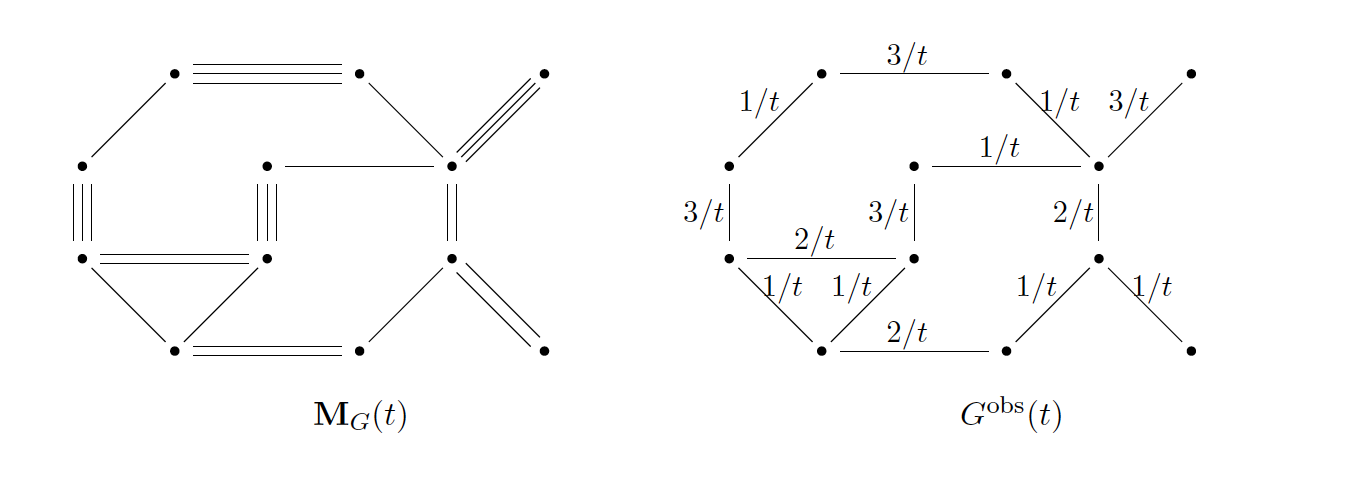
\includegraphics[scale=0.75]{Gobsrep}
  \caption{Observed Graph}
  \label{fig:gobsrep}
 \end{center}
\end{figure}


Note that in our setting the weights represent the strength of interaction, so this is not to be confused with weighed graphs where the $w_e$'s are regarded as cost.  In those cases we are oftentimes trying to minimize some aggregate quantity involving weights (such as travel distance, for example).  

\subsection{Estimating Functionals}

The setting we have formalized gives a clear mathematical problem.  Given functionals $\Gamma$ of interest, and $G^{true}$ unknown, what is the best way for us to estimate $\Gamma(G)$ given our observations of $G^{obs}(t)$. An immediate and naive frequentist approach is to first use $\frac{N_e(t)}{t}$ as an estimate of $w_e$, it is the maximum likilihood estimator.  This gives us $G^{obs}(t)$, a weighed graph which we use in place of the original to obtain $\Gamma(G^{obs}(t))$.  As natural as this definition is, we may be suspicious of $\Gamma(G^{obs}(t))$'s ability to approximate $\Gamma(G^{true}(t))$ in different regimes.  For instance, suppose a functional we care about is the total interaction rate of a vertex  $$ w_v := \sum_yw_{vy}$$  

Weighted graphs require a different distinction than the classic sparse\/dense dichotomy, one that is meaningful for weighted graphs.  For instance, even if a weighted graph  is complete it may have very small weights in all but an $O(1)$ number of edges--this scenario calls for a definition that can detect the sparsity of interaction despite a densely connected graph structure.  Define $$ w^* := \max_v w_v,$$ $$ w_*:= \min_v w_v.$$

For any sequence of graphs, we rescale the weights so that $w^* = \Omega(1)$, that is $\max_{v \in \mathcal{V}^{(n)}} w_v^{(n)}$ is bounded; this is a weighed graph version of bounded degree. We also assume $w_* = \Omega(1)$, so the graphs are connected.  Then

\begin{itemize}
    \item The \textbf{ diffuse} case occurs when $\lim_n \max_e w_e = 0$. 
    \item The \textbf{ local-compact} case where $\lim_{\epsilon \downarrow 0} \limsup_n \max_v \sum\{w_{vy}:w_{vy}\leq \epsilon \}=0$
\end{itemize}



If we had infinite time to observe the network, the naive Frequentist estimator we suggested would be a reasonable one.  In fact, there are three regimes of time that this problem can be broken down into.  

\begin{itemize}
    \item \textbf{ Short-term}: $t = o(1)$. This regime is too short and we have not yet seen an interaction at a typical vertex yet.  The only aspects of the unknown $G$ we can estimate relate to "local'' statistics of $O(1)$-size subgraphs (ex. triangles and other "motifs'' in the applied literature).  
    \item \textbf{ Long-term}: $t = \Omega(\log(n))$.  This  regime is enough observation time for the graph to be connected, typically.  Thus, at this point we can expect $\Gamma(G^{obs}(t))$ to be a good estimate of $\Gamma(G)$.  However, since the time required grows with $n$, in many applications, we do not have the luxury of such long observation times, especially with increasingly large graphs at our disposal for analysis.  
    \item \textbf{ Medium-term}: $t = \Theta(1)$.   This is a hard regime, and our project focuses here.  This regime in a real world is akin to saying that no matter how large the graph grows, we have finite time resources that cannot be scaled with the graph size $n$. A very likely constraint!
\end{itemize}
A compactness argument shows us that $w^{n}$ can be decomposed as a sum of a diffuse sequence and of a locally compact one.  So in that sense, the diffuse and local-compact weighted graphs form the dichotomy of limiting behaviour for weighted graphs.  

\section{Related Literature}
``Imperfectly-observed networks" has been studied from different viewpoints.  In the graph theory and complex networks literature, the treatment has mostly been on unweighted graphs.  We discuss here a couple of popular approaches in the literature and highlight how our approach is different.  

\begin{enumerate}
    \item Sampling vertices from a large graph and looking at their neighbourhood structure.  This approach aims to gather statistics of local structure in the graph.  One can see the algorithmic advantages of only gathering local data, and hence theory in the direction of inferring global guarantees from the local statistics are sought after.The paper \cite{Yaonan} gives a recent account of work in this direction.  The statistic they are concerned with is the degree distribution.  Which can be estimated from sampled data via the empirical degree distribution.  Yaonan et al. derive an estimator that performs much better under some contraints then using the naive empirical degree estimator.
    \item The area of link prediction is another perspective where after observing some revealed part of the network edges, we can produce a ranking of possible edges that exist in the true network. The ranking is based on the likilihood of these edges to be present given the observed data. This is a popular field, with obvious applications in recommendation systems.  The 2011 survey  \cite{link} on the topic of link prediction has been cited 752 times.
    \item Community detection in the Stochastic Blockmodel.  This area has some approaches that frame the problem as an imperfectly observed network problem.  For instance Jaewon et al. try to cluster real social networks by fitting a generative model via maximum liklihood to social network data in \cite{JureJaewon_overlapping_com}.  Since the networks are labelled, they can test their accuracy against other clustering algorithms. 
\end{enumerate}

To better illustrate how our regime is different from the above, let's dive deeper into what is being done in the degree distribution from sampling problem mentioned in 1.  In the framework in \cite{Yaonan}, they sample $k$ vertices and look at their degrees.  This gives them an estimate of the degree distribution, which has $O(1/\sqrt{k})$ independent of graph size $n$.  In our framework we are constrained by time.  Given $O(1)$ observation time, what can we observe?  Thus it doesn't make sense to talk about peering into all the edges of $k$ sampled vertices. A statistic that does make sense to talk about in the $O(1)$ observation time  regime is $w = \frac{1}{2}\sum_v w_v = \sum_e w_e$, the total edge density.  Another statistic in the weighted graph setting is the average vertex weight, given by $w = \frac{1}{2}\sum_v w_v = \sum_e w_e$.  We can try to estimate the distribution of $W := w_v$ for random $v \in V$.  A natural question to ask then, is what time frame is needed to give a good estimate of $W$?  

Let $$Q(i,t) = \text{ number of vertices with $i$ observed edges at time $t$}. $$

For $t = o(1)$ we have $$ \mathbb{E}Q(i,t) \equiv \frac{nt^i\mathbb{E} W^i}{i!}$$

In $t = \Omega(1)$ the mean number of observed edges that are repeated (so between the same two vertices) is about $\sum_ew_e^2t^2/2$.  So in our diffuse network , this ends up being only o(n) edges rather than $\Theta(n)$.  

Another point of difference is that, with the exception of the community detection example above, which sometimes involves analysis of the stochastic blockmodel as an artificial dataset to benchmark performance, the aforementioned areas of research do not involve a probability model.  The general line of reasoning is to first derive an algorithm, then compare to benchmarks established on real networks. Hence there is no hope for guarantees when dealing with real data, except for some measure of how well the application dataset mirrors the distribution of previous applications.

Our approach does not make assumptions on the underlying graph. It does so by first considering a weighted graph instead of a non-weighted one, and secondly demanding the theorems to be uniform over all edge weights.  This makes the framework very difficult, and perhaps not possible in many cases.  However the thesis moves in some very promising directions to obtain theorems of this flavour.  





\chapter{Estimators given by Large Deviation Bounds}

%Look at how actual functions you may care about can be different when predicted.  Get at some empirical data that shares this behaviour with your model. 

A lot of functionals of interest concern the maximum of the sum of edge weights.  In particular, they can be expressed in the form 
\begin{equation}
\Gamma(G) := \max_{A \in \mathcal{A}}\sum_{e\in A}w_e
\end{equation} 
where $\mathcal{A}$ can be any collection of edge sets.  For instance, if you wanted to find a subset of vertices of size $k$ that are highly connected (oftentimes the kind of property desired in a theoreticaly defined graph community), we can ask for $|\mathcal{A}| = k$. 

The naive estimator of the functional above, in the form $\Gamma(G^{obs}(t))$ given in the previous section, is particularly amenable to a large deviation bounds type argument because we are studying the maximum of a sum of independent Poisson random variables. Recall the large deviation bounds for $Poisson(\lambda)$ random variable are given by 
\begin{equation}
\begin{split}
\frac{\log \mathbb{P}(Poi(\lambda) \leq a\lambda)}{\lambda} &\leq -\phi(a), 0<a<1\\
\frac{\log \mathbb{P}(Poi(\lambda) \geq a\lambda)}{\lambda} &\leq -\phi(a), 1<a<\infty.
\end{split}
\end{equation}

Where $\phi(a)= a -1 -a\log a, \quad 0 < a < \infty$.
 
 \subsection{Weights of Communities}
 
 Community detection falls under the general umbrella of clustering problems.  The term community is motivated by social network applications, where nodes are people and communities capture the idea of a group of more interconnected people, for example, a group of people that share much more interactions than with people outside the group.  Naturally once this goal is specified, to find a community within a network is to optimize for interconnectedness.  A more in depth treatment of the clustering and community detection literature is given in Part II of this thesis.  
 
 A simple formulation in our graph terminology is to maximize the sum of the edge weights within a subset of fixed size:
 
\begin{equation}
w_m = \max\{\sum_{e \in A} w_e : |A^*|=m\}.
\end{equation} 
 
 Where $A^* \subset V$ and $A \subset E$ where A includes all edges where end-vertices are in $A^*$.  The maximum is taken over all vertex groups of cardinality $m$.  

We don't pay attention to computational cost and compute the naive frequentist estimator of $w_n$ via observing $G(t)$:

\begin{equation}
W_n(t) := \max\{ \sum_{e \in A} \frac{N_e(t)}{t} : |A^*| = m\}.
\end{equation} 

Since we are taking a max of a sum of independent variables, this sum will oftentimes be larger than the sum of their means, that is $W_e(t)$ tends to be larger than $w_m$.  In the case where the interaction rate at vertex $v$ denoted $w_v$ is O(1) and we fix $m$, $W_n(t) \rightarrow \infty $ as $n \rightarrow \infty$.  In this case, it's natural to normalize the total interaction in a community of size $m$ by the number of edges in the complete subgraph of size $m$.  In other words, we define community as $\frac{\sum_{e \in A} w_e}{m^2}$.  Communities of size $m$ thus exist if they are not $\frac{\sum_{e \in A} w_e}{m^2} \neq o(1)$ (so at least the pairwise interactions is at least constant order).  


 Note that $$Var (\frac{W_n(t)}{m^2}) = Var (\sum_{e \in \max A} \frac{N_e(t)}{t}) = \frac{w_m}{m^2\cdot t}$$ so the first order estimation error decreases as $\frac{1}{t^{1/2}}$ uniformly over $n$ and over weighted graphs (no dependence on $w_e$'s).

To get a hold of how our frequentist estimate behaves in the limit, suppose the size $m$ of communities we care about is order $\log(n)$:

By the union bound and using the fact that there are ${n \choose m}$ subsets of size $m$ in $G_n$, we arrive at:
\begin{equation}
\mathbb{P}(W_m(t) \geq \beta m) \leq {n \choose k} \mathbb{P}(Poi(w_m t) \geq \beta m^2 t).
\end{equation}


Given $w_m < \beta m^2$ we are in the position to apply large deviations bound  on $W_n(t)$ (since $\mathbb{E}(W_n(t)) = w_n$, we have

\begin{equation}
\begin{split}
\log \mathbb{P}(W_m(t) \geq \beta m) & \leq \log {n \choose m} -w_mt\phi(\frac{\beta m^2}{w_m}) \\
& \leq m \log n - w_m t \phi(\frac{\beta m^2}{w_m}) - \log m!.
\end{split}
\end{equation}

Our original assumption was that $m = \gamma \log n$, and set $w_m = \alpha m^2$ for some $\alpha < \beta$ (so we can still apply large deviation bounds), then

\begin{equation}
\log \mathbb{P}(W_n(t) \geq \beta m^2) \leq (\gamma - \gamma^2 \alpha t \phi(\beta/\alpha))\log^2n-\log m!.
\end{equation}

So if $\beta = \beta(\alpha, \gamma, t)$ is the solution of 
\begin{equation}
\gamma \alpha t \phi(\beta/\alpha) = 1
\end{equation}

then we can simplify the expression and tease out the asympotitics of the tail behaviour of $W_m(t)$ with

\begin{equation}
\mathbb{P}(W_m(t) \geq \beta m^2) \leq \frac{1}{m!}.
\end{equation}

This tells us that in the case of $m = \gamma \log n$ and outside of the event $\{ W_m(t) \geq \beta m^2\}$, which tends to $0$ as $n \rightarrow \infty$ as show in (2.9), we can bound the estimation error

\begin{equation}
\frac{W_m(t)-w_m}{m^2} \leq \beta - \alpha.
\end{equation}

Where $\alpha = w_m/m^2$ and $\beta$ given as the solution of equation (2.8).

The bound above is actually very general as it holds over all networks without assumptions on the distribution of weights $w_e$.  Another way to read this asymptotic bound is to consider how $\phi(a)$ behaves as $a \downarrow 1$. By taking the first two terms of its Taylor series expansion, $\phi(a) \sim \frac{(a-1)^2}{2}$ we get that

\begin{equation}
\beta - \alpha \sim \sqrt{\frac{2\alpha}{\gamma t}} \text{    as } t \rightarrow \infty
\end{equation}

We follow the frequentist setup of generating confidence intervals by assuming the existence of a true rate, and having hold of the distribution of observations. Thus, after observing the value of $\frac{W_n(t)}{m^2}$ we can be confident, based on the vanishing tail bound derived above, that $\frac{w_n}{m^2}$, our true community interaction rate, lies in the interval 

\begin{equation}
\Bigg[\frac{W_m(t)}{m^2}-\sqrt{\frac{2W_m(t)}{m^2\gamma t}}, \frac{W_m(t)}{m^2}+\sqrt{\frac{2W_m(t)}{m^2\gamma t}}\Bigg].
\end{equation}


\chapter{Maximum Matchings}
Suppose we have a weighted graph $G = (V, E)$ with an even number of vertices.  We can always assume $G$ is complete by assigning weight $0$ to edges not in $E$.  

\begin{definition}
A \textit{matching} is a set $\pi$ of $\frac{n}{2}$ edges such that each vertex is in exactly one edge. 
\end{definition}

\begin{definition}
The weight of a matching is given by $$weight(\pi, w):= \sum_{e \in \pi} w_e .$$
The \texit{maximum weight} is taken over all possible matchings: $$ \Gamma_1(w) := \max_{\pi} weight(\pi, w)$$ We care about maximal matchings because weights in our model indicate closeness (similar to how we maximized interactions in the previous section to define communities). 
\end{definition}
What can we say about estimating $\Gamma_1(w)$ by observing $G^{obs}(t)$ in our regime of interest of large but constant times $t = O(1)$? The naive estimator $\Gamma_1(G^{obs}(t))$ has several undesirable properties. Consider graphs $G^{true}$ with interaction rates of vertices $(w_v)$ of $O(1)$.  For locally compact graphs (where the intuition is that we do not have a growing number of small weighted edges per vertex) the matching $\Gamma_1(w)$ is of order $\theta(n)$.  In this case, the naive estimator may not perform so poorly, even though we construe $t$ as fixed, we still have growth in $n$, so the naive estimate improves as $n \rightarrow \infty$ \\

Suppose instead we observe a diffuse graph, an example of such a $G^{true}$ is the complete graph with $w_e = \frac{1}{n}$ for all edges $e$.  Then necessarily $\Gamma_1(w) = \frac{n/2}{n} = \frac{1}{2}$.  However, $G^{obs}$ is essentially the Erd\"os-R\'enyi random graph $\mathcal{G}(n, t/n)$. From results in \cite{David-incipientgiant} we have that $\Gamma_1(G^{obs}(t)) \sim c(t)n$ for a certain function $c(t)$.\\

So this is clearly incorrect.  Thus, if our $G^{true}$ contains a non-trivial component of a diffuse graph, we are in trouble when using the naive estimator, as it is off by a factor of $O(n)$.\\

We can circumvent the problem by reweighing the quantity of interest.  Consider $\frac{\Gamma_1(w)}{n}$.  This ratio can be read as the weight-per-vertex of the maximum-weight matching.  We can effectively ignore edges of weight $o(1)$.  We also consider edges for which we have observed at least two interactions.  

\begin{definition}\textit{Adjusted Vertex Weights}

\begin{center}

$weight_2 (\pi, G^{obs}(t)):= t^{-1}\sum_{e \in \pi}M_e(t)\mathbb{I}_{M_e(t) \geq 2}$\\
\bigskip


$\Gamma_2(G^{obs}(t)):= \max_{\pi} weight_2 (\pi, G^{obs}(t))$.

\end{center}
\end{definition}



This new definition will be useful if we can show that 
\begin{equation}
n^{-1}|\Gamma_2(G^{obs}(t)) - \Gamma_1(w)| \text{ is small for large } t \text{, uniformly over all } w.
\end{equation}

Note that we cannot do better than $O(t^{-1/2})$;  consider a graph with one edge.  Then we have an exact hold over the variance of the Poisson counts for one edge, which is of order $t^{1/2}$.  



\begin{prop}
\text{ Assume } $G^{true}$ \text{ satisfies } 

\begin{equation}
w_e \leq 1 \forall e \in E
\end{equation}

\text{ then } 
\begin{equation}
\mathbb{E}\bigg[n^{-1}(\Gamma_2(G^{obs}(t))-\Gamma_1(w)\bigg]^- \leq t^{-1/2} + \frac{1+\log t}{2 t},  \forall w \forall t \geq 1.
\end{equation} 

\text{ Assuming the even stronger condition of } 

\begin{equation}
w_v \leq 1, \forall v \in V
\end{equation}

\text{ we have } 

\begin{equation}
\bigg[n^{-1}(\Gamma_2(G^{obs}(t))-\Gamma_i(w)\bigg]^{+} \leq \Psi(t),  \quad \forall w
\end{equation}

\text{ where } 

\begin{equation}
\Psi(t) = O(t^{-1/2}\log t) \text{ as } t \rightarrow \infty
\end{equation} and $[\cdot]^+, [\cdot ]^-$ refer to the negative and positive portions respectively. 
\end{prop}

The proof works to bound $\Gamma_2(G^{obs}(t))$;  the contribution from small, i.e $o(1)$, weight edges can be controlled given our assumptions.  We prove a lemma that deals with it.  The contribution from $\Theta(1)$-weight edges can be controlled with large deviations type arguments because the assumptions limit the number of matchings with such weights to be exponential.  

\section{Bounding the Negative Contribution}

Here we derive the bound from the negative contribution in Proposition 1
$$
\mathbb{E}\bigg[n^{-1}(\Gamma_2(G^{obs}(t))-\Gamma_1(w)\bigg]^- \leq t^{-1/2} + \frac{1+\log t}{2 t},  \forall w \forall t \geq 1
$$

by finding a lower bound for $\Gamma_2(G^{obs}(t))$.

\bigskip

If we fix matching $\pi$, the sum of edge weights in the observed graph belonging to the matching is distributed as a Poisson random variable, since we are summing together independent Poissons.

$$ \sum_{e \in \pi} M_e(t) \sim \text{Poisson}(t\cdot weight(\pi, w)).$$ 

If we fix $\pi$ to be the matching attaining the maximum in 

$$\Gamma_1(w):= \max_{\pi} weight(\pi, w) $$

we get that 

$$ \Gamma_2(G^{obs}(t)) \geq weight_2(\pi, G^{obs}(t)).$$

This follows from the fact that $\pi$ is not necessarily the matching that attains the maximum for $\Gamma_2$, despite being the matching that attains the maximum for $\Gamma_1$.  

Thus to lower bound $ \Gamma_2(G^{obs}(t))$, it suffices to lower bound $weight_2(\pi, G^{obs}(t))$.  

Since $weight_2$ does not include contributions from edges that have less than 2 counts from $Poisson(w_e)$ we can rewrite the following difference as $$ \sum_{e \in \pi}M_e(t) - t\cdot weight_2(\pi, G^{obs}(t)) = \sum_{e \in \pi} M_e(t)1_{M_e(t)=1}.$$

Apply expectation on both sides gives us

$$ \mathbb{E}\bigg(\frac{\sum_{e \in \pi}M_e(t) - t\cdot weight_2(\pi, G^{obs}(t))}{t}\bigg)= \sum_{e \in \pi} w_e \exp(-tw_e).$$

Note that since $\pi$ attains the maximum for $\Gamma_1$, we actually have  
$$ \sum_{e \in \pi} M_e(t) \sim t \cdot \Gamma_1(w)$$.  

Our goal is to upper bound the right side using $0 \leq w_e \leq 1$ and $\sum_{e\in \pi}w_e = \Gamma_1(w) \leq n/2$.  To control different portions of the contribution from $w_e$ large and small, let's bound separately $w_e \leq b$ and $w_e > b$ for some b, which we choose a value for $b$  based on the final expression.  Immediately we have 

$$\sum_{e\in \pi}w_e\exp(-tw_e) \leq \frac{n}{2}b + \Gamma_1(w)\exp(-t b).$$

So to get the tightest bound we minimize the right side over $b > 0$.  This gives us

$$n^{-1}\sum_{e \in \pi}w_e \exp(-tw_e) \leq \frac{1}{2t}\psi(\frac{2t\Gamma_1(w)}{n})$$

where 
\begin{equation}
\begin{split}
\psi(x) &= 1+\log(x), x \geq 1\\
&= x,\quad  0 < x \leq 1.
\end{split}
\end{equation}


So to simplify the expression, if we defined $$D_2:= n^{-1}\bigg(t^{-1}\sum{e \in \pi} M_e(t) - \text{weight}_2(\pi, G^{obs}(t))\bigg) \geq 0$$

then we have shown that $$\mathbb{E}D_2 \leq \psi(\frac{2t\Gamma_1(w)}{n}).$$

Recall that $\sum_{e \in \pi}M_e(t)$  has $Poisson(t\cdot\Gamma_1(w))$ distribution, and since we were intersted in showing the difference in expectation of 
$$ D_1 := n^{-1}\bigg(t^{-1}\sum_{e \in \pi}M_e(t) - \Gamma_1(w)\bigg)$$ 

in the negative direction, so let us control 
$$ \mathbb{ P}(D_1 < \delta)  = \mathbb{P}\bigg(t^{-1}\sum_{e \in \pi}M_e(t) < t\Gamma_1(w) - nt\delta\bigg)$$.  

We can set $\lambda = t \Gamma_1(w)$ and $a = 1-n\delta/\Gamma_1(w)$ and use the first large deviations bound in (2.2), giving us

$$\mathbb{P}(D_1 < -\delta) \leq \exp(-t\Gamma_1(w)\phi(1-n\delta)).$$

And since $\phi(1-\eta) \leq \eta^/2$, we can further simplify to 

$$ \mathbb{P}(D_1 < -\delta) \leq \exp(\frac{tn^2\delta^2}{2\Gamma_1(w)}).$$

But by assumption $\frac{\Gamma_1(w)}{n}\leq 1/2$ and $n \geq 2$ so we get 

$$\mathbb{P}(D_1 < -\delta) \leq \exp(-2t\delta^2). $$

Integrating over $\delta$ gives us 
$$\mathbb{E}\min(0, -D_1) \leq 2^{-3/2}\pi^{1/2}t^{-1/2}. $$

So using the estimates from $D_1$ and $D_2$ we are able to lower bound $D$:

\begin{equation}
\begin{split}
D &:= n^{-1}\big( \Gamma_2(G^{obs}(t))-\Gamma_1(w))\big)\\
&\geq n^{-1}\big(\text{weight}_2(\pi, G^{obs}(t))-\Gamma_1(w))\big) = D_1-D_2.
\end{split}
\end{equation}

So 

\begin{equation}
\begin{split}
\mathbb{E}\max(0, -D) &\leq \mathbb{E}\max(0, D_2-D_1)\\
&\leq \mathbb{E}D_2+\mathbb{E}\max)0, D_1)\\
&\leq 2^{-3/2}\pi^{1/2}t^{-1/2} +\frac{1}{2t}\psi(t)
\end{split}
\end{equation}

using also that $\Gamma_1(w) \leq n/2$.  This implies the first lower bound cited in Proposition 1.  

\section{The Upper Bound}

If we fix a matching $\pi$, the sum of our edge counts in $\pi$ given by $\sum_{e \in \pi}M_e(t)$ has Poisson$(t \cdot \text{weight}(\pi, w))$ distribution.  since $\text{weight}(\pi, w)) \leq \Gamma_1(w)$ we can use the second large deviations bound given at the beginning of the chapter, with $\lambda = t \cdot \Gamma_1(w)$ to get

$$ \frac{1}{t \cdot \Gamma_1(w)}\log \mathbb{P}\bigg( \sum_{e \in \pi} M_e(t) \geq nt(\frac{\Gamma_1(w)}{n}+a)\bigg) \leq -\phi(1+\frac{an}{\Gamma_1(w)}), a >0.$$

Multiplying $1/n$ by both sides and rearranging some terms within and outside of $\mathbb{P}$ we get 

\begin{equation}
n^{-1}\log \mathbb{P}\bigg( n^{-1} \sum_{e \in \pi} M_e(t)/t \geq \frac{\Gamma_1(w)}{n}+a\bigg) \leq -tn^{-1}\Gamma_1(w)\phi(1+\frac{an}{\Gamma_1(w)}), a >0.
\end{equation} 

Which will be easier for us to parse in terms of the following matchings.  For $k\geq 2$ let $\Pi_k$ be the set of partial matchines $pi$ that only use edges with weight greater than $1/k$, and suppose that the matchings are maximal with respect to this constraint (i.e they are the largest matchings given all $w_e > 1/k$).  Since we have paths of length $n$ and we have at most $k$ such $w_e$ to choose from, if we had more we would violate the assumption that total weight is less than $1$. From this we can at infer $|\Pi_k| \leq k^n$.  Note that if we take any matching $\pi$ (doesn't have to be from $\Pi_k$), the subset of edges with $w_e > 1/k$ still form part of a partial matching in $\Pi_k$, so it follows from $|\Pi_k| \leq k^n$ and (3.10) that 

\begin{multline}
n^{-1}\log \mathbb{P}\bigg( \exists \pi \in \Pi_k: n^{-1} \sum_{e \in \pi, w_e > 1/k}M_e(t)/t \geq \frac{\Gamma_1(w)}{n}+a\bigg)\\ \leq -tn^{-1}\Gamma_1(w)\phi(1+\frac{an}{\Gamma_1(w))+\log k}).
\end{multline}

To control the contribution from the low weight (less than $1/k$) edges let us define

$$ \Delta_k(\pi):= \sum_{e \in \pi, w_e \leq 1/k}M_e(t)1_{M_e(t) \geq 2}.$$

But by definition a matching uses only one edge per vertex so we can bound this using $M^*_v := \max\{M_{vy}(t):w_{vy} \leq 1/k\}$ to get

\begin{equation}
\max_{\pi}\Delta_k(t) \leq \frac{1}{2}\sum_vM_v^*1_{M_v^* \geq 2} 
\end{equation}

\begin{lemma}
Let $(N_i, i\geq 1)$ be independent Poisson($\lambda_i)$, and write $N^* := \max_i N_i$. Suppose $s:=\sum_i\lambda_i \geq 1$ and choose $lambda^* \geq 1$ such that $\max_i\lambda_i \leq \lambda^* \leq s$.  Then we have

$$\mathbb{E}N^*1_{N^*\geq 2} \leq C \lambda^* (1+\log(s/\lambda^*)) $$ for some constant $C$.  
\end{lemma}

\begin{proof}
Given at end of section.
\end{proof}

To apply Lemma 3.2.1 we note that  $M_{vy}(t)$ has Poisson$(tw_{vy})$ distribution and \\
$\sum_{u:w_{vy} \leq 1/k} w_{vy} \leq 1$ by our assumption that 
$w_v \leq 1, \forall v$.  So regarding $s=t$ and $\lambda^* = t/k$ gives us the lemma result that 

$$ \mathbb{E}M^*_v1_{M_v^* \geq 2}\leq Ctk^{-1}(1+\log k),\qquad k \leq t$$

Applying (3.12) gives us 

\begin{equation}
\frac{1}{n}\mathbb{E}[\max_{\pi}\Delta_k(\pi)] \leq \frac{1}{2}Ctk^{-1}(1+\log k),\quad k \leq t
\end{equation}

We are trying to upper bound 

$$ D:= n^{-1}\big( \Gamma_2(G^{obs}(t)) - \Gamma_1(w)\big)$$

so let us call the event in the probability in (3.10) $B$.  By definition, $B^c$ is the event that 

$$  n^{-1}\Gamma_2(G^{obs}(t)) \leq n^{-1}\Gamma_1(w) + a +n^{-1}t^{-1}\max_{\pi}\Delta_k(\pi).$$

So this gives us

$$ D \leq a + n^{-1}t^{-1}\max_{\pi}\Delta_k(\pi).$$

Let $F$ be the event that $\{n^{-1}t^{-1} \max_{\pi}\Delta_k(\pi) > a\}$ then the above simplifies to 

$$ D < 2a, \text{ on } B^c \cap F^c$$

and from Markov's inequality and 3.13 we have $$\mathbb{P}(F) \leq Ck^{-1}(1+\log k)/a, k \leq t.$$

Summing up, 3.10 gave a bound on $\mathbb{P}(B)$, we just gave a bound on $\mathbb{P}(F)$, and also dervied a bound on $B^c \cap F^c$.  So putting these together we get 

\begin{equation}
P(D > 2a) \leq \exp(n(-tn^{-1}\Gamma_1(w)\phi(1+\frac{an}{\Gamma_1(w)}) + \log k))+Ck^{-1}(1+\log k)/a, \quad k \leq t.
\end{equation}

Our goal now is to optimize over the choice of $k$.  

Let us continue the calculations using leading terms to clarify the exposition.  In particular we use the asymptotic relation $\phi(1+\delta) \sim \delta^2/2, \delta \downarrow 0$.  This allows us to simplify the term, along with using $\Gamma_1(w) \leq 1/2$

$$\Gamma_1(w)\phi(1+\frac{an}{\Gamma_1(w)})= \frac{a^2n}{2}\frac{n}{\Gamma_1(w)}  \geq a^2n .$$

This allows us to rewrite 3.14 as 

\begin{equation}
\mathbb{P}(D > 2a) \leq k^n \exp(-nta^2) + Ck^{-1}(1+\log k)/a, k \leq t.
\end{equation}

Most notably, this bound does not depend on $w$!  Integrating over $a$ allows us to get an expression in terms of $\mathbb{E}(D)$. 

\begin{equation}
\int_{a_0}^1 \mathbb{P}(D > 2a)da \leq k^n \frac{1}{2nta_0} \exp(-nta^2) + Ck^{-1}(1+\log k)\log{1/a_0}
\end{equation}

Recall that $k$ was our parameter to separate the big $w_e$ and small $w_e$, where we isolated the contribution from $w_e \leq 1/k$.  If we now set $k = t$ and $a_0 = t^{-1/2}\log t$ for large $t$ our bound becomes


\begin{equation}
\int_{a_0}^1 \mathbb{P}(D > 2a) da \leq \frac{\exp(-n(\log^2t - \log{t}))}{2n^{1/2}\log t} + \frac{C \log^2 t}{t}
\end{equation}

The right hand side is in fact uniformly bounded in $n$ by a function that decays as $o(t^{1/2})$ as $t \rightarrow \infty$.  

So 

$$ \int_{a_0}^1 \mathbb{P}(D > 2a)da = o(t^{-1/2}) \text{ as } t\rightarrow \infty, \text{ uniformly in } n $$

So finally we have 

$$ \mathbb{E}D^+ = 2\int_{a_0}^1 \mathbb{P}(D > 2a)da +\int_{2}^{\infty} \mathbb{P}(D > a)da $$

The last term we are able to control because $D \leq n^{-1}\Gamma_2(G^{obs}(t))$ and clearly $\Gamma_2(G^{obs}(t)) \leq t^{-1}\sum_eM_e(t)$ since any matching is bound by the total sum.  

But $\sum_eM_e(t)$ has Poisson($t\sum_eM_e(t)$) distribution so by the assumption that $w_v \leq 1 \forall v$ we have that 

\begin{center}
D is stochastically smaller than $\frac{1}{nt}$Poisson($nt/2$)
\end{center}

So using the large diviation upper bound stated at the beginning of this chaper we can conclude that $\int_{2}^{\infty} \mathbb{P}(D > a)da \rightarrow 0$
exponentially fast in $nt$.  Thus the asmptotic behaviour of $\mathbb{E}D^+$ is dominated by the first term, which means it is $O(t^{-1/2}\log{t})$ as $t \rightarrow \infty$, uniformly in $n$.  

\begin{proof}\textit{Lemma 2.}


Recall that Lemma 2 states that given $(N_i, i\geq 1)$ are independent Poisson($\lambda_i)$. Suppose that $N^* := \max_i N_i$. Suppose $s:=\sum_i\lambda_i \geq 1$, and suppose we choose $\lambda^* \geq 1$ such that $\max_i\lambda_i \leq \lambda^* \leq s$.  Then we have
\begin{center}
$$\mathbb{E}N^*\mathbb{1}_{N^*\geq 2} \leq C \lambda^* (1+\log(s/\lambda^*)) $$ for some constant $C$.  
\end{center}

Let's regard $N_i$ as the counts of a rate-1 Poisson point process on the interval $[0,s]$ in successive intervals of lengths $\lambda_i$.  Let $k = \ceil*{s/\lambda^*}$  be successive intervals of length $\lambda^*$.  By definition of $\lambda^*$, each intervals in the first collection must be contained in the union of two successive intervals in the second collection.  This observation allows us to simplify our proof, since it would be sufficient to prove that there exists a constant $C$ such that if $(N_i, 1 \leq i \leq k)$ are i.i.d Poisson($\lambda^*$) with $\lambda^* \geq 1$ and 

$$ \mathbb{E}N^*1_{N^* \geq 2} \leq C \lambda^* (1+\log{k})$$

Clearly, if $\lambda^* \geq 1$ there is some constant $B$ such that for $i \geq B \lambda^*$

$$ \frac{\mathbb{P}(Poisson(\lambda^* \geq i+1))}{\mathbb{P}(Poisson(\lambda^* \geq i))}.$$

Using this for the last step in the inequality below we have 

\begin{equation}
\begin{split}
\mathbb{E}N^* &= \sum_{i \geq 1}\mathbb{P}(N^* \geq i)\\
 &\leq \sum_{i \geq 1} \min (1, k\mathbb{P}(Poisson(\lambda^*) \geq i))\\
&\leq 1 + \max(B\lambda^*, \min \{ i: \mathbb{P}(Poisson(\lambda^*) \geq i) \leq 1/k\}).
\end{split}
\end{equation}

Finally by the large deviations uppers bound we have that there exists $C^* < \infty$ such that 

$$  \mathbb{P}(Poisson(\lambda^*) \geq i) \leq 1/k, \lambda^* \geq 1, i \geq C^* \lambda^* (1+ \log k).$$
\end{proof}

\chapter{Concentration Inequalities for Observed Multigraph Process}

\section{Markov Chain Preliminaries}

Recall that a discrete state Markov Chain is a sequence of random variables $X_1, X_2, X_3...$ with the property that the probability of moving to the next state only depends on the previous state.  This is commonly referred to as the Markov property.  More formally $$ \mathbb{P}(X_{n+1} = x | X_1 = x_1, X_2 = x_2, ..., X_n = x_n) =P(X_{n+1} = x | X_n = x_n)$$ where $x, x_i \in S$, the countable state space of possible values of $X_i's$.  

\section{Multigraph Process Formulation}

Recall that our weighted graph model can also be construed as a multigraph process by looking at the multigraph induced by the Poisson counts of the Poisson random variable with mean given by the edge weights.  More formally, let $m = (m_e, e\in E)$ be a multigraph on a given vertex set $V$.  Here we let $m_e \geq 0$ denote the number of copies of edge $e \in E$ that links vertices in $V$.  Our model naturally associates an observed multigraph process denoted by $$(M(t), 0 \leq t < \infty) = (M_e(t), e\in E, 0 \leq t < \infty).$$

Note that this is a continuous time Markov chain.  It's state space is the set $\mathbb{M}$ of all multigraphs over $V$ where the transition rates $$ m \rightarrow m \cup \{ e\}, \text{  are given by rate   } w_e.$$
\bigskip
where $\psi(x)$
\bigskip

\begin{definition}\textit{Standard Process}

The Markov chain given by $(M(t), 0 \leq t < \infty) = (M_e(t), e\in E, 0 \leq t < \infty)$, where  $M(t)$ starts from the empty set $\emptyset.$
\end{definition}

\begin{definition}

Multigraph Monotonicity Property

Let $$ T = T_{\mathcal{A}} = \inf \{t : M(t) \in \mathcal{A}\}$$ be the stopping time where $\mathcal{A} \subset \mathcal{M}$ is the set of multigraphs such that $$ \text{ if } m \in \mathcal{A} \text{ then } m \cup \{e\} \in \mathcal{A}, \forall e.$$

For the chain started at some state $m$, define $$ h(m): = \mathbb{E}_mT_{\mathcal{A}}.$$



By the monotonicity property we have that the hitting time of a set in $\mathcal{A}$ is lower bounded by the hitting time of sets above it in the chain.  That is

\begin{equation}
h(m\cup \{e\}) \leq h(m).
\end{equation}

\end{definition}

Naturally then, starting from $\emptyset$ will give $h(\emptyset)$ that upper bounds all such $h(m)$. 

In this setting we can quote the following concentration bound from \cite{david_FFP}.

\begin{prop}[\cite{david_FFP}]
For the standard chain, for a stopping time $T$ defined above we have $$ \frac{var T}{\mathbb{E}T} \leq \max_{m, e}\{h(m) - h(m \cup \{e\}) : w_e > 0\}$$
\end{prop}

Two examples of such a stopping time where we can estimate the bound well with the appropriate monotonic proces: 

$$ T^{tria}_k : = \inf\{t: M(t) \text{ contains k edge-disjoint triangles}\} $$

$$ T^{span}_k := \inf\{t: M(t) \text{ contains k edge-disjoint spanning trees} \}$$

\begin{prop}[\cite{david_FFP}]

Let s.d. denote the standard devation. 

$$ \frac{s.d.(T^{tria}_k)}{\mathbb{E}T^{tria}_k} \leq \bigg( \frac{e}{e-1}\bigg)k^{-1/6}, k \geq 1$$

$$ \frac{s.d.(T^{span}_k)}{\mathbb{E}T^{span}_k} \leq k^{-1/2}, k \geq 1$$

\end{prop}

This is a setting in which the above bounds actually do not depend on $w$, so it is uniform over all weighted graphs.  

This bound will be useful for obtaining an estimator of a functional when we have a stopping time $T$ that is concentrated around its mean that also does not depend on $w$.  In that case we will be able to use the proposition to provide a bound uniform over all $w$ of some functional $\Gamma(w)$ defined by the expectation of the stopping time.   

The proof of the proposition requires special structural properties of spanning trees and triangles.  The technique for triangles also hold for analogs of similar subgraphs. The question of whether this argument can apply to "k copies of substructure" is open, however it does not apply as easily in all cases.  In section we show a case in which the argument does not apply easily.

For proposition 2 to be useful, we need $ \max_{m, e}\{h(m) - h(m \cup \{e\}) : w_e > 0\}$ to be bounded.  If we instead require $\{h(m)-h(m\cup \{e\})$ be bounded for the most possible transitions, it is possible to obtain applications of the monotonicity argument to first-passage percolation\cite{david_FFP} and the appearance of a incipient giant component in in-homogenous bond percolation\cite{david_FFP}.  These problems lie outside the current framework.  

In this multigraph Markov chain setting, our stopping times $T$ also satisfy the submultiplicative property

\begin{equation}
\mathbb{P}(T > t_1+t_2) \leq \mathbb{P}(T > t_1)\mathbb{P}(T>t_2),\quad t_1, t_2 >0.
\end{equation}

%We can easily see this by considering the set of events that require at least $t_1+t_2$ hitting time, and recognize it is a subset of those that require both $t_1$ and $t_1$

Submultiplicative properties of random variables are know to give a right exponential tail bound:

\begin{equation}
sup\{\mathbb{P}(\frac{T}{\mathbb{E}T} > t : T \text{ submultiplicative } \} \text{ decreases exponentially as } t \rightarrow \infty
\end{equation}

We can also bound the left tail by iteratively applying the monotonicity property to get $\mathbb{P}(T < k t_1) \leq \mathbb{P}(T > t_1)^k$, which gives us 

\begin{equation}
\begin{split}
\mathbb{E}T &\leq \frac{t_1}{\mathbb{P}(T \leq t_1)}\\
\mathbb{P}(T \leq t_1) &\leq \frac{t_1}{\mathbb{E}T}\\
\mathbb{P}(T \leq a \mathbb{E}T) &\leq a, 0 <a <1.
\end{split}
\end{equation}
By setting $t_1 = a \mathbb{E}T$.

In other words, if our stopping time $T$ enjoys the submultiplicative property (4.2), then after observing the value of $T$ in the observed process 
\begin{equation}
\text{ we can be } (1-a) \text{-confident that } \mathbb{E}T \leq T/a \text{ in the true process }. 
\end{equation}

Note that Markov's inequalty, which states that $\mathbb{P}(T \geq a) \leq \frac{\mathbb{E}T}{a}$ gives us a different confidence statement, namely that $$ \text{ we can be } (1-a) \text{-confident that } \mathbb{E}T \geq aT.$$

\section{Measuring Connectivity via Multicommodity Flow}

A key open problem in our framework is to prove a result of the following type.  Given our observation time is large, but of order $t = O(1)$, the observed $G^{obs}(t)$ will have a giant component of some size, say $(1-\delta)|V|$.  However, this graph may not be completely connected.  We want a statement that allows us to conclude that $G$ enjoys a "well-connected" connectivity property within a large subset of its vertices if we observe that $G^{obs}(t)$ has a "well-connected" property within its giant component.  

Recall that the graph Laplacian is a well studied way to quantify connectedness in graphs.  In particular, the spectral gap gives bounds for many quantities that relates to the connectedness qualities of a graph.  We discuss the Laplacian in detail in part II of this thesis so don't provide definitions here.  

Proving bounds on the spectral gap in our regime without assumptions on $w$ is quite difficult.  However to give a push towards results of this flavour, we provide a result not in terms of connectedness as quantified by spectral gap, but by measuring connectivity in terms of the existence of flows whose magnitude is bounded relative to edge-weights.  Note that our observed graph $G(t)$ may very well be disconnected in the time regimes of $t=O(t)$, so we cannot hope to get a flow between all vertex pairs in $G$.  Instead our definition must use information of flows between \textit{most} pairs. 

\begin{definition}
A \textit{path} between vertex $x$ to vertex $y$ is a set of directed edges that connects $x$ to $y$; a \textit{flow}, denoted by $\phi_{xy} = (\phi_{xy}(e), e \in E)$ is a vector indexed by edges of a path, where each $\phi$ is given by 

$$\phi_{xy}(e) := \nu \mathbb{P}(e\in \gamma_{xy}) $$

where $\gamma_{xy}$ is some random path from $x$ to $y$.  We let $|\phi_{xy}|$ denote the volume $\nu$ of a flow.  
\end{definition}

\begin{definition}


A \textit{multicommodity flow} $\Phi$ is a collection of flows $  (\phi_{xy}, (x,y) \in V \times V)$ (including flows of volume zero).  We let $$ \Phi[e] := \sum_{(x,y)}\phi_{xy}(e)$$ denote the total flow across edge $e$.  

\end{definition}
Let's consider the following function on the network.  Suppose $\Phi$ is constrained by the following:

\begin{equation}
\text{The volume } |\phi_{xy}| \text{ is at most }n^{-2}, \text{ where }(x,y) \ in V\times V
\end{equation}

\begin{equation}
\Phi[e] \leq \alpha w_e.
\end{equation}

The first condition allows us to somewhat normalize the total flow, whereas the second let's us control how much flow flows through edge $e$ via its weight.  

\begin{definition}
$$\Gamma_{\alpha}(w) := \max_{\Phi \text{satisfies two conditions above}}\sum_{(x,y)\in V\times V} |\phi_{xy}|.$$
\end{definition}

By our conditions, $\Gamma_{\alpha}(w) \leq 1$. The smallest $\alpha$ for which $\Gamma_{\alpha}(w) = 1$ also bounds the spectral gap. This is known as the canonical path or Poincar\'e method\cite{persi}.\\

Let's define the $(\alpha, \delta)$-properly to hold if $\Gamma_{\alpha}(w) \geq 1 - \delta$.  If we have the property holds for small $\delta$, we are quantifying via lower bounding the flow that the network has a well-connected component. As $\alpha \downarrow$ and $\delta \downarrow$, our property becomes stronger and the degree with which it has a large well-connected component is also larger. 

Returning back to the observed networks framework we aim to prove a statement of the form: If $G^{obs}(t)$ has $(\alpha, \delta)$-property, then we are 95\% confident that the unknown $G^{true}$ has $(\alpha^*, \delta^*)$-property for some $(\alpha^*, \delta^*)$ independent of $w$.  

Let $$T_{\alpha, \delta} := \inf \{ t: \Gamma_{\alpha}(M(t)) \geq 1-\delta\}.$$
where we interpret the multigraph $M(t)$'s edge count as integer edge-weights.  

$M(T)$ by definition allows a total flow of volume greater than $1-\delta$, and by assumption satisfies the normalizing property (4.5) as well as the analogue of property (4.6) for the multigraph (using $ N_e(t)/t \sim w_e$). If we take expectations over realizations of $M(T)$ we get $\Gamma_{\alpha}(w) \geq 1-\delta$ and furthermore 

$$ \Phi[e] \leq \alpha \mathbb{E}M_e(T) = \alpha w_e \mathbb{E}T, \text{ for all } e.$$

Recall Wald's inequality, which applies to a sequence $(X_n)_{n \in \mathbb{N}} $ of independent identically distributed random variables. If $N$ is some non negative integer valued random variable we have 

$$ \mathbb{E}(X_1+...+X_n) = N \mathbb{E}(X).$$

Applying this to $M_e(t) = N_e(t)/t$ we get that 

$$ \Phi[e] \leq \alpha \mathbb{E}M_e(T) = \alpha w_e \mathbb{E} T. $$

So summarizing, we were able to derive from $G^{obs}$ satisfying (4.5) and the analogue of (4.6) that $$ G^{True} \text{ has the } (\alpha\mathbb{E} T, \delta) \text{ property}$$

But we have just shown in the last section in (4.5) that we can be $(1-a)$ confident that $\mathbb{E}T \leq T/a$.  So it follows that 

\begin{equation}
\text{ we are } (1-a)-\text{confident that } G^{true} \text{ has the }(\alpha T/a, \delta)-\text{property}.
\end{equation}

\section{Logic of Inference between Observation and Truth}

Though we are quite used to citing confidence intervals in statistical jargon, it is worth spending some time spelling out the underlying logic of the inference being made. Though it follows basic forms of inference, it's worth discussing here as it may seem intuitive to want proofs along the lines of wanting to establish desirable properties in the observed graph given desirable properties in the real graph.  However the correct direction of the inference is in fact the converse of that. Particularly in the context of our applications, this inference appears counter-intuitive.  To formalize:

Suppose $P$ is some property of a network we care about.  The statements we wish to prove follow the inference format 
\begin{center}
If $G^{obs}$ has property $P$ then we are $\geq 95\%$ confident that $G^{true}$ has property $P^*$.
\end{center}

Where $P^*$ is reasonably related to $P$.  For instance, both measure connectedness.  To prove a statement of the above form, we actually need a theorem of the following form (using the contrapositive):

\begin{center}
\textit{Theorem}: if $G^{true}$ does not have property $P^*$ then with $\geq 95\%$ probability $G^{obs}$ does not have property $P$.  
\end{center}

The reason for using the contrapositive is because it would be very difficult to enumerate all instances of graphs with property $P$, so instead we assume the negation of the conclusion and deduce that the observed graph cannot have property $P$.  

What this means for our program is that in order to establish desirable properties in our random graphs, we work in its negative form.  So for instance in the case of $P$ representing connectivity properties of the graph, we must show that given the true graph is not well connected, the observed graph cannot be either.  We are not showing that the observed graph is well connected given the true graph is (converse).  Happily, this is typically false in our time scale as well.  

\chapter{First Passage Percolation}



The first passage percolation (FPP) literature has been an extremely well studied on in probability theory.  Though originally inspired by models of water percolating in soil, the general field, which is characterized by studying paths in a random medium.  Nowadays the field's theorems lend themselves well to studying the spread of information over networks, such as virality in social networks, or actual pathologies in a biological network.  The notion of first passage percolation is formulated as follows in our setting.  

\begin{figure}[h]
\begin{center}
  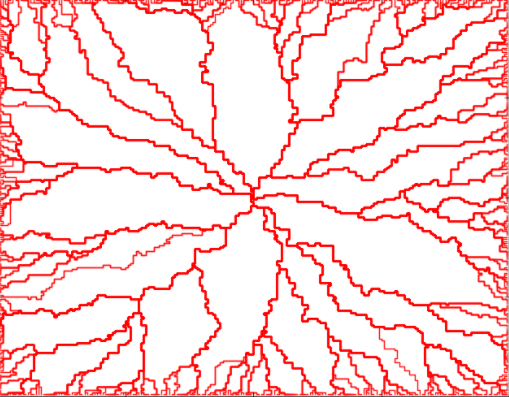
\includegraphics[width=0.45\textwidth]{fpp.png}
   \caption{First passage percolation to the boundary of a lattice graph with exponential edge weights. Figure taken from \cite{wiki}.}
 \end{center}
\end{figure}

Let $G = (V, E, w)$ be a network and suppose $u, v$ are two distinct vertices in $G$.  Let $\xi_e \sim \text{Exponential}(w_e)$. We interpret our weights $w_e$ as the parameters of these random edge traversal times.  The random first passage percolation time from $u$ to $v$, denoted by $X(G)$, is the minimum value of $\sum_{e\in \pi}\xi_e$ over all paths $\pi$ from $u$ to $v$.  Note the that is not necessarily achieved by the path that minimizes $\sum_{e\in \pi}w_e$ since $\xi$ is a random variable so even though some paths may have greater total weight sum, there is still a small probability that the traversal time realization can be smaller than that of a smaller total weight path.  Hence $X(G)$ is a random FPP.  

The functional that interests us in this setting is $$ \Gamma(G) : = \mathbb{E}X(G).$$

Note that to estimate $X(G)$ from the observed process, we actually have two layers of randomness here.  First the randomness contribution from $X(G)$ (which we smooth over with $\mathbb{E}$) and then a contribution from $N_e(t)$, the multi-edges of $G^{obs}$.  

The following lemma gives us an idea of how $X(G^{obs})$ relates to $X(G)$.
In particular to study the functional $\Gamma$ we use the following lemma. 

\begin{lemma}
$$\mathbb{P}(X(G^{obs}(t)) \geq x) \geq \mathbb{P}(X(G) \geq x),\quad 0 < x<\infty .$$
\end{lemma}

Let's tease out why this lemma is phrased in such a way.  For any fixed $t$ we have $\mathbb{P}(X(G^{obs}(t)) = \infty) > 0$ since $v$ and $u$ may not be in the same connected component since the edges arrive as a Poisson process in $G^{obs}$.  Note this is trivially true if $u,v$ not connected, so we are assuming $u$ and $v$ are connected in $G^{true}$.  So estimation procedures should involve the stopping time for when $u$ and $v$ are connected.  The lemma unfortunately does not extend easily to stopping times.  

\begin{proof}
The unconditional distribution of $X(G^{obs}(t))$ is the distribution of FPP times for which edge-traversal times $\xi_e^*(t)$ are independent with distributions given by:\\
the conditional distribution of $\xi_e^*(t)$ given $M_e(t)$ is $ \text{Exponential}(M_e(t)/t)$, where Exponential($a$) denotes the exponential distribution with parameter a. So it is sufficient to show that $\xi^*_e(t)$ stochastically dominates Exponential($w_e$) distribution of $\xi_e$.  

We have

\begin{equation}
\begin{split}
\mathbb{P}(\xi_e^*(t) \geq x) &= \mathbb{E}(\mathbb{P}(\xi_e^*(t) \geq x |N_e(t))\\
&= \mathbb{E}(\exp(-x N_e(t)) \\
&\geq \exp(-x \mathbb{E}(N_e(t)/t))\\
&=\exp(-x w_e)\\
\end{split}
\end{equation}
where the last step follows by Jensen's inequality. 
\end{proof}

\section{A General Conjecture Fails}

Observing $G^{obs}$ will eventually give us a good estimate of $X(G)$, since we can simulate it from $G^{obs}$ once $t$ is large enough that its own FPP process is distributed as $X(G)$. That is, it is clear that 

\begin{equation}
\text{ On every network } G \text{ we require at most } O(\Gamma(G)) \text{ observation time. }
\end{equation}


One may expect however, that for certain types of networks, in particular with a more constrained geometry, we may be able to estimate $\Gamma(G) := \mathbb{E}X(G)$ quicker than having to wait for such a stopping time. Consider the linear graph $G$ as an example.  It is a naturally example since the FPP between edges are much simpler, in fact it is by necessity the path the unique path that connects two nodes. Suppose $G$ has $m$ edges where each edge weight is of order $\Theta(1)$.  Then instead of having to wait for $\Theta(m)$ time in order to , we simply have to wait for $N_e(t)/t$ to be good estimators for $w_e$, which occurs in $\Theta(\log m)$ time (by arguments following from the coupon collector's process).  Another candidate for such an observation time is the following stopping time, inspired from Proposition 3 (section 4.2).  

\begin{equation}
T_k := \inf \{t: M(t) \text{ contains k edge-disjoint paths from } u \text{ to } v\}.
\end{equation}

Where $k$ is large and fixed.  This is a natural candidate since the reason why $\Gamma(G)$ is hard to calculate is because we need to take the infimum over many different paths.  However, a result in this direction is not likely.  Our argument below offers an explanation why.  

\begin{center}
\textbf{Claim:} For any estimator satisfying (5.2), the observation time required must be $\Theta(\Gamma(G))$ for every $G$.  
\end{center}

To see this, let $G_n^{1}$ be a network with $n$ two-edge routes running between vertices $v^*$ and $v^{**}$.  And let the edge weights on all edges in these routes be $n^{-1/2}$.

\begin{figure}
\begin{center}
  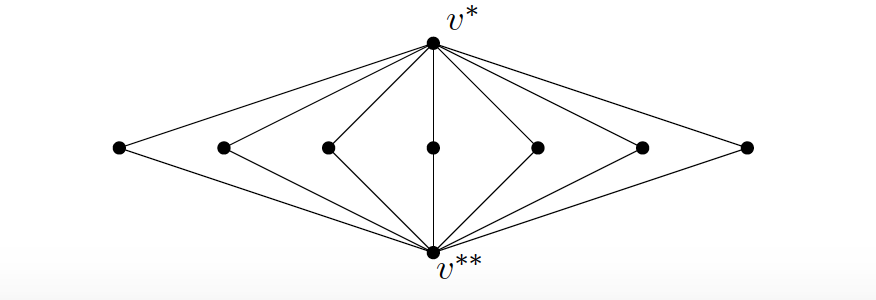
\includegraphics[scale=0.75]{manypaths}
  \caption{Network $G^1_$}
  \label{fig:many_paths}
 \end{center}
\end{figure}



In this case, the observation stopping time defined in 5.3 requires as much time as the FPP time for $\Gamma(G_n^1)$.  Now if we had an estimator that satisfies 5.2, it would have to decide whether to stop at time $t$ or continue observing.  If the decision were based on $M(t)$ it should only use the subset of $M(t)$ that consists of paths from $v^*$ to $v^{**}$.  Suppose by way of contradiction that we have an estimator that requires observation time $\tilde{T}_n << \Gamma(\tilde{G}_n)$.  Let's rescale the edge weights so we can normalize their times so that $\tilde{T}$ is $o(1)$ and $\Gamma(\tilde{G}_n)$ is $\Omega(1)$.  We can now create a new graph $G_n$ which is the union of $\tilde{G}_n$ and $G^1_n$ (by identifying vertices with the same index and taking the union of edges).  Now if we wait $\tilde{T}_n$ time as dictated by graph $\tilde{G}_n$, it will sometimes see the same subset of edges that we would have seen in the case of observing $G^{obs}$ corresponding to $\tilde{G}_n$.  At that point we are in the same empirical position as we would have been if $G^{true}$ were $\tilde{G}_n$, so we would be confident enough to stop observing, as in the case of $\tilde{G}_n$.  However the availability of the many paths to choose from in $G^1_n$ requires that $\Gamma(G_n)$ is in fact $\Theta(1)$.  In other words, we need to observe much longer to get the true min of all passage times. So we we really were incorrect in stopping our observations, since $G$ is a union of $G^1_n$ and $\tilde{G}_n$.  


\part{Graph Clustering with Graph Neural Networks}

\chapter{Clustering on Graphs}

Finding clusters is an important task in many disciplines, whether to uncover hidden functional similarities in protein interaction networks, to compress data, or to improve ecommerce recommendations. The second part of this thesis studies how we can use neural networks to do clustering on graphs.  

\begin{figure}[H]
\begin{center}
  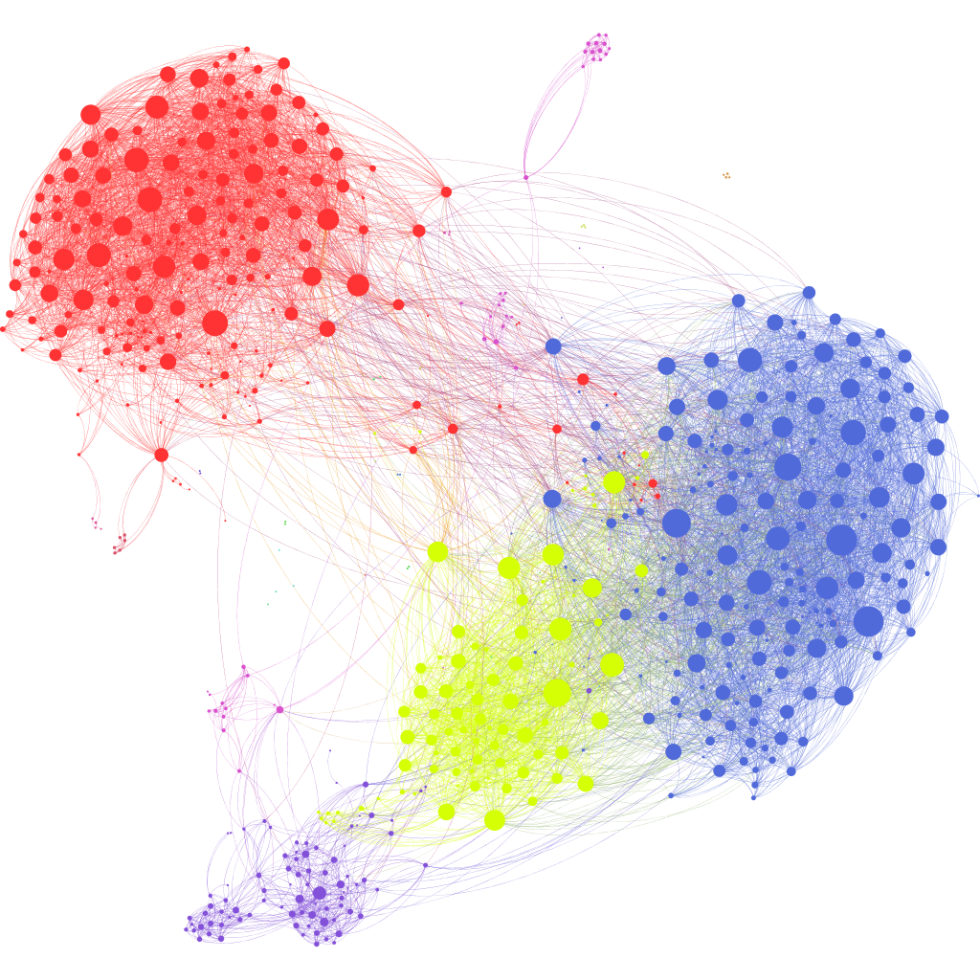
\includegraphics[scale=0.13]{social_network.png}
  \caption{A sampling of a Facebook friend network.\cite{social_network}}
  \label{fig:socialnet}
 \end{center}
\end{figure}

Clustering is a procedure applied to datasets in which we output a community label for each vertex.  All vertices that have the same label are referred to as cluster. Points within a cluster share some kind of similarity, more so with each other than with points outside the cluster. The definition is not precise because clustering can span the spectrum between supervised (eg. community detection with ground truth) and unsupervised problems (eg. data exploration). Graph clustering is the clustering procedure applied to a dataset that has graph structure. The goal here is to use the extra topological information of the network to do clustering and inform choices of similarity measures.


Applied to social networks, clustering is oftentimes referred to as community detection. The procedure can be data driven or model driven.  In the former we let the  features in datasets motivate definitions of similarity metrics and even suggest ground truth.  In the latter, a probabilistic generative model is often used, where the generative mechanism defines the ground truth communities.  The two approaches are not unrelated.  Generative models, for instance, are designed to mimic statistics of real graphs.  The Stochastic Blockmodel is an example of such a benchmark artificial dataset and we will discuss it in detail.  




\begin{figure}
\begin{center}
  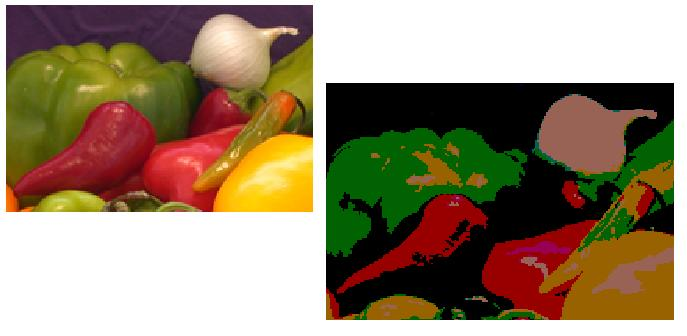
\includegraphics[scale=0.35]{image_segmentation.jpg}
  \caption{A result of image segmentation.\cite{image_seg}}
  \label{fig:seg}
 \end{center}
\end{figure}

\begin{figure}
\begin{center}
  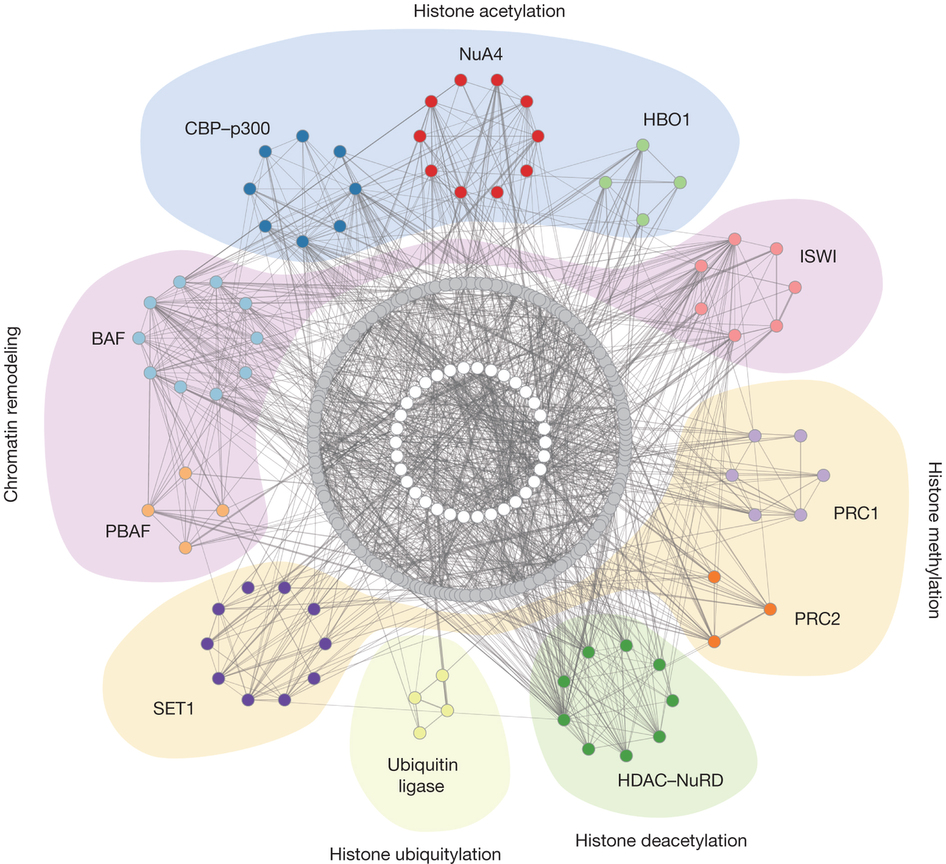
\includegraphics[scale=0.20]{protien_network.jpg}
  \caption{A protein to protein interaction network.\cite{protein}}
  \label{fig:protien}
 \end{center}
\end{figure}



The benefit of the neural network approach is that we do not have to choose what algorithm to use via heuristics or local statistics gathered from the network.  Instead it is data driven.  The model will learn by gradient descent, fitting the best parameters given the distributions of the graphs it learns from.  We will first go over the well studied Stochastic Blockmodel and some of the algorithmic challenges of community detection in this model. Then we will introduce the Graph Neural Network, a model we designed that can successfully do clustering on the SBM, even in the hardest regimes.  We will present our experimental results in the last section.  


\chapter{A Primer on Clustering in the SBM}

Two challenges before us in studying clustering procedures rigorously are: 
\begin{center}
What is the ground truth?\\

What are the algorithmic guarantees?
\end{center}
Approached from a theoretical point of view, progress on these questions comes from studying special cases, oftentimes derived from generative probability models that capture much of the empirical behaviour.  One extremely well studied model is the Stochastic Blockmodel (SBM).  One quick Google scholar search reveals about 8000 papers written on this topic, around 3000 of which since 2014.  It's a particularly simple and natural extension of the Erd\H{o}s Renyi random graph model, which exhibits community structure.  The randomness involved in the construction of the graph allows one to prove properties of the graph that hold asymptotically.  Despite the simplicity of its definition (requiring few parameters), the SBM has proved fertile grounds for testing algorithmic performance.  Theoretical questions to do with community detectability thresholds for the model given certain parameters have only been addressed in the easiest of regimes (2 communities)  in the last couple of years, using techniques ranging from branching processes in probability theory to phase transitions in Ising-like models in statistical physics.  

\begin{definition}The \textit{Stochastic Block Model (SBM)} is a random graph model that can be defined by the following three parameters.
\begin{align*}
    n & : \text{ The number of vertices in the graph. }\\
    c & =(c_1, ...c_k): \text{ A partition of the vertex set,} \{1,2, ...,n\} \text{, into } k \text{ disjoint subsets. }\\
    W & \in \mathbb{R}^{k \times k}_{\geq 0}: \text{A symmetric matrix of probabilities of connections between the } k \text{ communitites.}
\end{align*}

Given the above parameters, one can sample a SBM$(n, c, W)$ graph, call it $G = (V, E)$ (where $V$ is the vertex set and $E$ is the edge set, and $n= |V|$) by connecting two vertices $u, v \in V$ with probability $W_{ij}$, where $W_{ij}$ is the $ij^{th}$ entry of $W$, $v \in c_i$ and $u \in c_j$.  Whether one edge is in the SBM or not is independent of other edges and is solely determined by $W$ and $c$.  
\end{definition}

In the easiest case with two communities of the same size, we can define the SBM with 3 scalar paramters $n$, $p, q$, where $n$ is the number of vertices, $p$ is the probability of connecting two vertices if they are from the same community and $q$ is the probability of connecting between two nodes of different communities. 


Since the SBM is a random graph, a given set of parameters will give rise to a distribution of graphs.  For instance, the following three graphs come from the same parameters: $n = 8$, $c = (\{0,1,2,3\}, \{4,5,6,7\})$, and $W =([1,0.15],[0.15,1])$. Otherwise put, in the simpler $3$-scalar parametrization, we have that Figure \ref{fig:awesome_image1}, \ref{fig:awesome_image2} and \ref{fig:awesome_image3} are all instantiations of SBM with parameters $p=1.0$, $q=0.15$ and $n=8$.  
\begin{figure}[h]
\minipage{0.32\textwidth}
  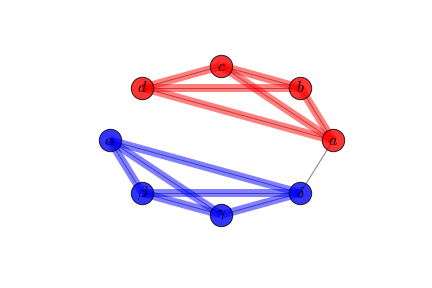
\includegraphics[width=\linewidth]{labels_and_colors_1.png}
  \caption{Instantiation 1 of SBM with $p=1.0$, $q=0.15$.}\label{fig:awesome_image1}
\endminipage\hfill
\minipage{0.32\textwidth}
  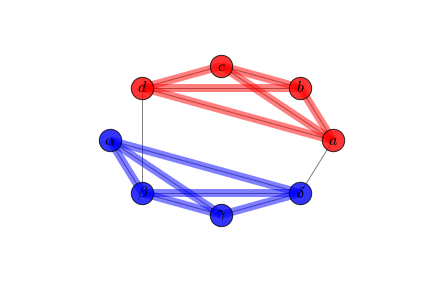
\includegraphics[width=\linewidth]{labels_and_colors_2.png}
  \caption{Instantiation 2 of SBM with $p=1.0$, $q=0.15$.}\label{fig:awesome_image2}
\endminipage\hfill
\minipage{0.32\textwidth}%
  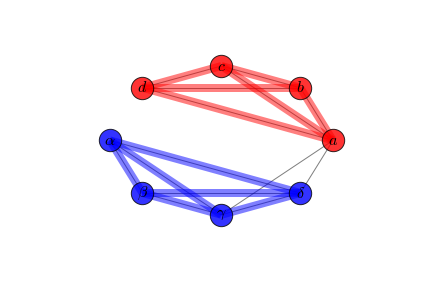
\includegraphics[width=\linewidth]{labels_and_colors_3.png}
  \caption{Instantiation 3 of SBM with $p=1.0$, $q=0.15$.}\label{fig:awesome_image3}
\endminipage
\end{figure}


So why is the clustering on the SBM hard?  Clusterings for the instantiations above can be convincingly eye-balled.  Let's consider another example.  

\begin{figure}[h]
\begin{center}
  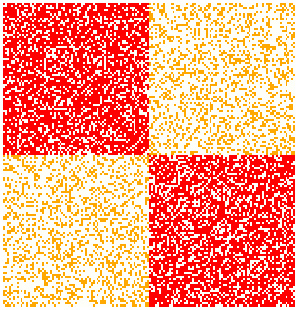
\includegraphics[scale=0.5]{SBM}
  \caption{Coloured and ordered adjacency matrix of SBM. Figure taken from \cite{SBM_adjacency_talk}}
  \label{fig:SBM_matrix_colour}
 \end{center}
\end{figure}

The figure \ref{fig:SBM_matrix_colour} is a coloured adjacency matrix representation of an SBM graph. Here we represent the adjacency matrix by colouring a square in \ref{fig:SBM_matrix_colour} if there is an edge, and leaving it white if there is no edge.  The red and yellow colouring differentiates the different community membership relationships (red for edges that are between two nodes of the same community, and yellow for edges between nodes that differ in their community membership). The number of nodes $n$ is much bigger in \ref{fig:SBM_matrix_colour} than in \ref{fig:awesome_image1}. Clearly $p$ and $q$ also don't seem too far apart, since the density of red and yellow nodes, though the difference is still perceptible, is not a great difference.  In a real clustering problem we don't know the actual colouring, as in the case in \ref{fig:SMB_uncolored}.

\begin{figure}[h]
\begin{center}
  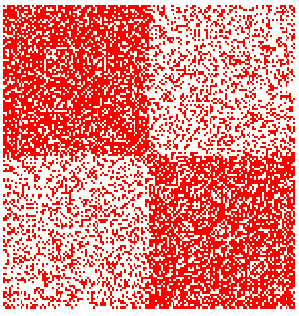
\includegraphics[scale=0.5]{SMB_uncolored}
  \caption{Ordered by uncoloured SBM adacency matrix.  Figure taken from \cite{SBM_adjacency_talk}}
  \label{fig:SMB_uncolored}
 \end{center}
\end{figure}

And most importantly, we don't actually know the order of the nodes as we cannot in \ref{fig:SMB_unordered}.  As in the previous two representations of the same graph, we ordered the nodes so that the nodes of one community proceed the other.  Of the $n\!$ permutations, there's only a few that makes that true, a diminishing small percentage of the total possible number of orderings of $n$ nodes.  

\begin{figure}[h]
\begin{center}
  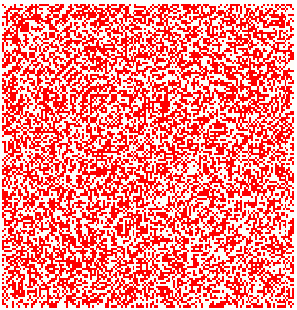
\includegraphics[scale=0.5]{SBM_unordered}
  \caption{Uncoloured and unordered adjacency matrix of SBM.  Figure taken from \cite{SBM_adjacency_talk}}
  \label{fig:SMB_unordered}
 \end{center}
\end{figure}

In \ref{fig:SMB_unordered} we don't have any hope of eyeballing all possible partitions of this graph into two communities.  

\section{Regimes of Clustering: Sparse to Dense}

One of the things \ref{fig:SBM_matrix_colour}, \ref{fig:SMB_uncolored}, and \ref{fig:SMB_unordered} help highlight is how much more difficult clustering can be if the difference between $p$ and $q$, the in-community probability of connecting and out-community probability of connecting (respectively), is small.  In fact, there is a rigorous quantification of this heuristic, as it drives a dichotomy in the quality of community recovery we can achieve. 
To talk about asymptotic behaviour of the SBM, let's confine our discussion to the the balanced SBM with two communities.  The definitions are easily extendable to SBM in general, however focusing on this balanced two community SBM makes clear what is being held constant and what is growing when we talk about asymptotic behaviour. 


\begin{definition}
We say a clustering of SBM(n, p, q) gives an \textit{Exact Recovery} if the probability of estimating the correct cluster assignments on SBM(n,p,q) goes to one as the number of nodes $n$ grows.  A clustering of the nodes $\{1, 2, ..., n\}$ is a partition of the nodes into communities.  We can encode that as a binary valued function $F : V \rightarrow \{0,1\}$ in the case of the two community SBM(n, p, q). So the exact recovery regime can be stated as $$\mathbb{P}( F_n = \bar{F_n}) \rightarrow_n 1.$$  Where $F_n$ corresponds to the correct clustering for SBM(n, p, q) and $\bar{F_n}$ is the predicted cluster assignments.   
\end{definition}

\begin{definition}
We say the clustering of SBM(n,p,q) gives \textit{detection} of the true communities if the predicted clusters correlate with the true communities.  Using the same $F_n$ (true community assignments) and $\bar{F_n}$ (predicted community assignments) as above, that means $$\exists \epsilon > 0 : \mathbb{P}(|F_n-\bar{F_n}| \geq 1/2+\epsilon) \rightarrow_n 1.$$ To adapt this definition to SBMs with $k$ communities, the $1/2$ inside the probability changes to $1/k$.  
\end{definition}

A key thing to understand here is that the detection regime is not just a weaker regime, it is actually impossible to have exact recovery for some families of $\{$SBM(n,p,q)$\}_n$.  Consider for instance when the SBM is not connected. In that case, the isolated vertices would have underdetermined community membership.  See \ref{fig:sparse} for a diagram of such an SBM. Furthermore, achieving detection of the true communities is not even possible for certain choices of $p,q$ of the  $\{$SBM(n,p,q)$\}_n$ as well.  The bulk of results in \cite{MNS} investigate what sparse regimes of the 2 community SBM can we only hope for partial recovery. They show this by proving in a very precise sense that correlating the a particular node's community membership with its neighbours is impossible, thus showing there is an information theoretic impossibility to even detection.  


\begin{figure}[h]
\begin{center}
  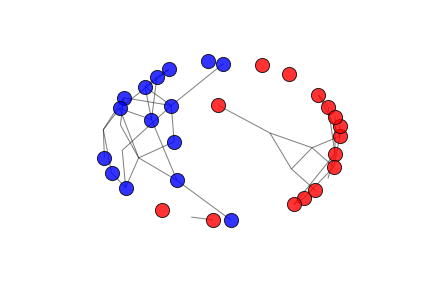
\includegraphics[scale=0.5]{SBM_balanced_large_sparse.png}
  \caption{Underdetermined labels due to isolated vertices.}
  \label{fig:sparse}
 \end{center}
\end{figure}

\subsection{Algorithmic Challenge}

In terms of the algorithmic challenge, the optimization problem is quite clear.  We are trying to find a graph partition that satisfies the minimum cut problem.  This problem is famously known to be $NP$-hard. If we constrain the problem to only consider balanced communities (communities of the same size) the problem becomes $NP$-complete.  For large $n$ graphs, we want to do better than just brute force go through all possible partitions.  Here relaxing the problem has presented many opportunities to apply spectral algorithms, semi-definite programming and belief propagation methods.  Since spectral methods have been shown to achieve the information theoretic threshold mentioned in the previous section, and because it provides the inspiration for our Graph Neural Network model, we will give an exposition of spectral clustering algorithms here.  

\section{Spectral Clustering for the SBM}

Spectral clustering is based on studying the spectrum of the graph Laplacian.  


Let $G= (V, E)$ be a graph, possibly weighed graph where $\{w_{ij}\}$ are the weights.  The degree of vertex $v_i$ is given by 
$$ d_i := \sum_{j=1}^n w_{ij}.$$

The degree matrix $D$ then is the diagonal matrix with entries $d_1, ..., d_n$ along its diagonal. Let $W$ be the adjacency matrix of $G$.  

\begin{definition}The \textit{unnormalized graph Laplacian} is defined as

$L : = D-W.$ 
\end{definition}
\begin{definition}The \textit{symmetric graph Laplacian} is defined as

$L_{sym} : = I - D^{-1/2}WD^{-1/2} = D^{-1/2}LD^{-1/2}.$ 
\end{definition}
\begin{definition}The \textit{random walk Laplacian} is defined as

$L_{rw} : = I - D^{-1}W = D^{-1}L.$ 
\end{definition}

The graph Laplacians above enjoy some nice properties.  In particular: 

\begin{prop}{\cite{tutorial_SC}}
\begin{itemize}
    \item For every $v \in \mathbb{R}^n$ we have
    $$v L v^T = \frac{1}{2}\sum_{i,j =1}^nw_{ij}(v_i-v_j)^2.$$
    \item $L$ is symmetric and positive semi-definite.
    \item The smallest eigenvalue of $L$ is 0, the corresponding eigenvector is the constant one vector \textbf{1}. $0$ is also an eigenvalue of of $L_{rw}$ and $L_{sym}$, corresponding to the constant one vector \textbf{1} and $D^{-1/2}$as eigenvectors respectively. 
    \item $L$ has $n$ non-negative, real-valued eigenvalues $0 = \lambda_1 \leq \lambda_2 \leq ...\leq \lambda_n$. 
\end{itemize}
\end{prop}

 Spectral clustering algorithms generally use some version of graph Laplacians, either one of the three classical ones above, or some matrix that is a perturbation of a Laplacian.  We will discuss one such perturbation when we define the Bethe Hessian matrix in the next chapter.  As for the steps of a generic spectral clustering algorithm, it follows roughly the following steps.  

\begin{algorithm}[H]
 \KwData{A graph adjacency matrix $W$ corresponding to graph $G = (V, E)$. Let $k$ be the number of clusters desired.}
 \KwResult{A clustering of the vertices $v$ into $k$ clusters.  This can be encoded as a function $F: V \rightarrow \{1,2,...,k\}$.}
 \begin{enumerate}
    \item Create $L$, $L_{sym}$, $L_{rw}$ from $W$.  Let us call the matrix we are finding the spectrum of $Q$. 
    \item Take eigendecomposition of $Q$.  
    \item Take the $k$ dimensional eigenspace associated with biggest or smallest eigenvalues of Q. Choose the eigenspace corresponding to the biggest eigenvalues if $Q = L$, and the eigenspace corresponding to the smallest eigenvalues if $Q= L_{sym}$ or $Q = L_{rw}$.  
    \item Project the vertices $v \in V$ onto this $k$ dimensional subspace.
    \item Perform the k-means algorithm on the projected vertices. 
    \item Done. 
 \end{enumerate}
 \caption{General Spectral Clustering Algorithm}
\end{algorithm}


Choosing what matrix to use for $Q$ is somewhat of an art in clustering problems, especially when it comes to applying it to real data.  In the case of generative models, we have a better understanding of what the cuts should look like.  Are we minimizing cuts while normalizing by volume?  Is our graph extremely sparse that the extreme eigenvalues exhibit large fluctuations?  In short, there are many versions of spectral algorithms that depend differ on what matrix the spectral algorithm is applied to.  A bulk of them is based on the Laplacian, some on other matrices we can derive from the adjacency matrix of a network. 

One way of seeing how spectral clustering works is to regard the spectral decomposition as a particularly useful embedding of $v \in \mathbb{R}^n$ (as represented by the adjacency matrix) to $\bar{v} \in R^k$ (where $k$ is how many clusters we want to extract).  The eigenbasis is informative because it provides us the most extreme directions that highlights where connections are most sparse (the eigenproblem is in fact a relaxation of min cut).  For instance, consider an instantiation of SBM($n =40, (p = 0.5, q = 0.05)$).  Here $k = 2$.  In \ref{fig:randomproj} and \ref{fig:spectralproj} we compare a random projection of our vertex set to $\mathbb{R}^2$ with a projection using the spectral basis.  

\begin{figure}[h]
\minipage{0.4\textwidth}
  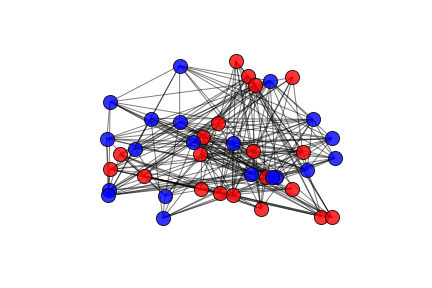
\includegraphics[scale=0.6]{SBM_balanced_large_dense_rand.png}
  \caption{Random Embedding}
  \label{fig:randomproj}
\endminipage\hfill
\minipage{0.4\textwidth}
  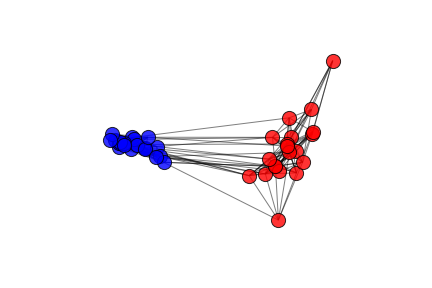
\includegraphics[scale=0.6]{SBM_balanced_large_dense_spectral.png}
  \caption{Spectral Embedding}
  \label{fig:spectralproj}
\endminipage\hfill
\end{figure}

\section{Thresholds for Detectability and Exact Recovery}

If we wish to talk about regimes of recovery, we need to use the constant degree parametrization so that we can talk about sparse and dense graphs.  In particular, in the two balanced community SBM$(n,p, q)$ we can reparametrize with $a :=  p \cdot n$ and $b := q \cdot n$.  Where $a, b$ are the average within-community and out-of-community average degrees respectively.  The regimes where exact recovery and detection can be made are the following. 

\begin{itemize}
    \item \textbf{Exact Recovery}:$p=\frac{alog(n)}{n}, q = \frac{b log(n)}{n}$.  Recovery if and only if $\frac{a+b}{2} \geq 1 + \sqrt{ab}$.
    \begin{itemize}
        \item In \cite{MNS} Mossel, Neeman, and Sly provide a polynomial time algorithm that is capable of recovering the parameters in the exact recovery threshold (the threshold which they prove below which no algorithm can recover the communities).  The proof has three stages. First classical spectral clustering is to compute an initial guess. A replica stage is then used to reduce error by holding out subsets and repeating spectral clustering on remaining graph.  And finally, on a small number of uncertain labels, majority rule to refine their assignments. 
         \item Abbe, Bandeira and Hall show in \cite{ABH} that they can provide an algorithm using semi definite programming to achieve the state of the art in the same sparse regime as above. 
    \end{itemize}
    \item \textbf{Detection}: $p = \frac{a}{n}, q = \frac{b}{n}$.  Detection iff $(a-b)^2 > 2(a+b)$.
    \begin{itemize}
        \item Mossel, Neeman and Sly show in \cite{MNS_sparse} that they can do partial recovery with spectral clustering with initial guess, then finish the algorithm with belief propagation to refine the guess.  \\
        \item Massoulie showed in \cite{Massouli} that spectral clustering can be applied successfully in this regime using the non-backtracking matrix, a matrix that counts the number of non backtracking paths from each vertex of a given length.   \\
        \item Saade, Krzakala and Zdeborová showed in \cite{AFL} that a type of deformed Laplacian via a 1-dim parameter that shares eigenvalues with non-backtracking matrix for spectral decomposition can be used successfully in this regime.  This deformation Laplacian is called the Bethe Hessian.    
    \end{itemize}
   \end{itemize}
   
This list serves to highlight several things.  First that the results are all very recent. And also that the results are not trivial, it took a lot of hard work and ingenuity from mathematicians, statisticians, physicists and theoretical computer scientists to prove them.  The proofs require tools form random matrix theory, the theory of branching processes and semi definite programming, to name a few, so a fairly deep level of machinery and theory was required. Also, notice that in each regime there is a successful algorithm that can achieve the theoretical threshold with a spectral approach.  The only catch is what type of matrix to apply the spectral method to.  Thus the takeaway is that there is no one size fits all model. Clustering, even in the two community case of the SBM takes a lot of expertise to define the right kind of parameters and matrices whose spectrum will amplify the right signals given the regime of the SBM parameters.  

Given all this, the present work's contribution is the following.  We will design a neural network architecture that is expressive enough to approximate these spectral algorithms.  Show that it can replicate the state of the art in SBM regimes, especially noteworthy are the difficult sparse regimes where we graze the information theoretic threshold. % And finally, perhaps most importantly, show that these models can be applied successfully to real data, and provide a computationally efficient approach.
In sum, the goal of bringing neural networks to bear on the problem is to let gradient descent replace the "ingenuity" aspect of clustering.  We no longer need to meticulously choose the right matrices to apply spectral clustering to.  Gradient descent will learn the correct parameters, in a data driven way. 

\chapter{The Graph Neural Network Model}


\section{Graph Neural Network}

The Graph Neural Network (GNN) is a flexible neural network architecture that is based on two local operators on the a graph $G = (V, E)$. Given some input signal $F \in \mathbb{R}^{n \times p}$ on the vertices of an n-vertex graph, we consider two operators that acts locally on this signal as well as a non-linearity.\\


\noindent D: Diagonal matrix of degrees of $V$.  Define $(DF)_i = deg(i) \times F_i$.  \\
W: Adjacency matrix of $G$.  Define $(WF)_i:= \sum_{j\sim i }F_j.$\\
\textbf{$\theta$}: Pointwise Non-Linearity For each layer of the graph neural network, and for each node, we have $\eta_{\theta}: \mathbb{R}^p \times \mathbb{R}^p \rightarrow \mathbb{R}^q$ parametrized by $\theta$ trainable. Thus each node $i \in G$ undergoes $g_i = \eta_{\theta}(((DF)_i, (WF)_i)$\\


\begin{figure}
\begin{center}
  \includegraphics[width=\textwidth]{GNN.png}
  \caption{An example of an architecture constructed from operators D, W and $\theta$}
  \label{fig:GNN}
 \end{center}
\end{figure}

Immediately from this definition, we get that after one layer of applying $D$ and $W$ allows us to recover the graph Laplacian operator.  To be precise, let $F$ be a $p$-dim signal on $G$.  Then if we define $$ \eta(DF, WF) := DF - WF$$ we recover the unnormalized graph Laplacian.  If we allow ourselves preprocessing to also define $D^{-1/2}$ and $D^{-1}$, we will be able to recover the symmetric and random walk Laplacians.  Furthermore, by stacking together several of the Laplacian modules, and allowing ourselves to renormalize the signal after each  module, we are able to recreate the power method.  Therefore the expressive power of this architecture includes approximations to eigendecompositions.\\

\subsection{Related Work}
The GNN was first proposed in \cite{GNN} as a way to approximate functions on graphs. Bruna et al. also generalized convolutions for signals on graphs\cite{Bruna}.  The idea there is that the convolution neural network architecture so successful for image data, can be construed as decomposing the image signals into the very rapidly decaying Fourier basis.  Rapidly decaying because images lie on such regular graphs (in particular grids). The right generalization is then to use the graph Laplacian's eigenbasis to create a general graph convolution.  The authors successfully applied this neural network for signals on meshes.  Kipf and Welling showed more recently in \cite{kipf2016semi} the GNN with a symmetric Laplacian module, with only two layers can be quite effective as a embedding mechanism for graph signals.  And applied their network to semi-supervised learning problems where some graph nodes were labelled but others were not.\\

The present work is the first time a neural network has been applied to community detection.  In particular this means the graphs we are dealing with are far larger and far sparser then all previous works.  The GNN architecture family is quite general, so it required taking the most expressive combination of modules to include in it's expressive closure spectral algorithms of interest mentioned in the last chapter.  We are able to show that our version of the GNN can compete with spectral algorithms in doing spectral clustering on the SBM in even the hardest of regimes (detectability).  This will not work with previous GNN architectures mentioned above.  In addition, we are not doing an eigendecomposition, which is required of spectral algorithms.  Thus making the network more efficient computationally.  %Lastly we apply the GNN to extremely large graphs, with millions of nodes.  These real datasets have ground truth communities which we compare the performance of.  




\chapter{Experiments}
\section{Artificial Datasets}

\subsection{Spectral Clustering on the Bethe Hessian for the SBM}
\begin{definition}The 
\textit{Bethe Hessian} is a one parameter perturbation of the unnormalized graph Laplacian.  Let $D$ be the diagonal matrix of degree of graph $G$ and $\mathbb{I}$ be the identity matrix in $n$ dimensions (where $G$ has $n$ vertices).  We define the Bethe Hessian as a matrix that depends on $r \in \mathbb{R}$ as  $$BH(r) := (r^2-1)\mathbb{I} - rA +D.$$
\end{definition}

Saade et al. showed in \cite{AFL} that the Bethe Hessian was a competitive matrix to do spectral clustering on when close to the information theoretic threshold of detection of $a,b$ for the SBM.  It has the benefit of being easily computed from the adjacency matrix. Recall that the information theoretic threshold for SBM($n, a/n, b/n)$ occurs for bounded degree graphs $G$ when $(a-b)^2 = 2(a+b)$.  When $(a-b)^2 > 2(a+b)$ we can recover the communities, when $(a-b)^2 < 2(a+b)$ we cannot.  Saade et al. did an experiment to compare bounded degree graphs with average degree 3, and compared various spectral methods, as well as belief propagation with spectral clustering on the Bethe Hessian. The best $r$ to use for the Bethe Hessian was motivated by results in statistical physics, it was empirically shown to give good accuracy for $r$ equal to the root of the average degree of the graph in the case of the SBM, but in general requires one to solve an eigenproblem on the graph zeta function.  See \cite{AFL} for details. 

\begin{figure}[h]
  \begin{center}
  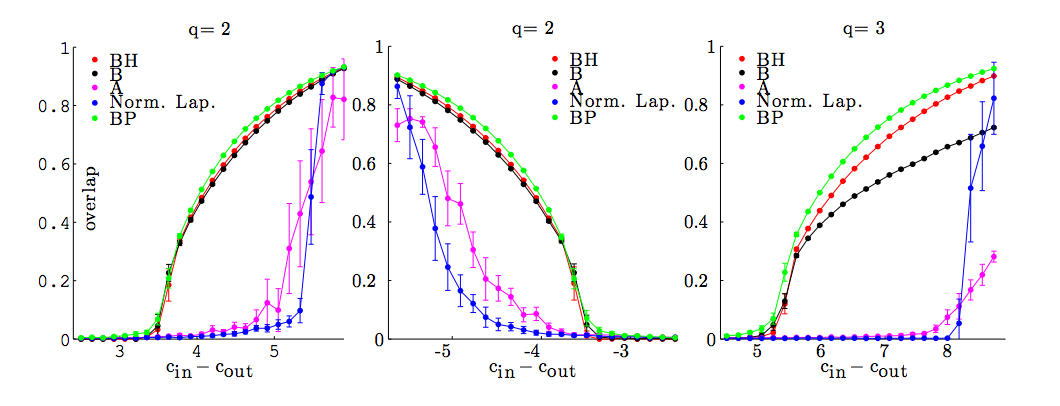
\includegraphics[scale=0.4]{BH_SBM.png}
  \caption{Spectral clustering with the Bethe Hessian compared to other popular methods that work at the limit of clustering detectability. Average degree of all SBM graphs is 3 (extremely sparse regime). This graph of results is taken from \cite{AFL} and shows the optimality of using BH, allowing spectral methods to be efficient even at the informational theoretic boundary of this problem.}
  \end{center}
\end{figure}

Our first experiment is to see if the GNN can learn the optimal scalar $r$ such that spectral clustering with $BH(r)$ becomes informative. Of course, since $r$ is a scalar, it is more efficient to brute force search for the solution rather than use gradient descent. However this preliminary experiment is meant to show that gradient descent can retrieve the optimal $r$ given the GNN architecture's ability to approximate the power method in order to find the eigenvectors of $BH(r)$.  

To be clear, the experimental task is as follows.

\begin{itemize}
    \item Input: Adjacency matrices A (instantiated from specific $SBM(n,a/n, b/n)$). 
    \item The parameter to be learned via gradient descent is $r$ of $BH(r)$. 
    \item Output: A community assignment of vertices ($F : V \rightarrow \{0,1\}$. 
    
\end{itemize}

The model was able to decrease loss, converge and get close to the theoretically verified optimal $r$. 

\begin{figure}
\begin{center}
  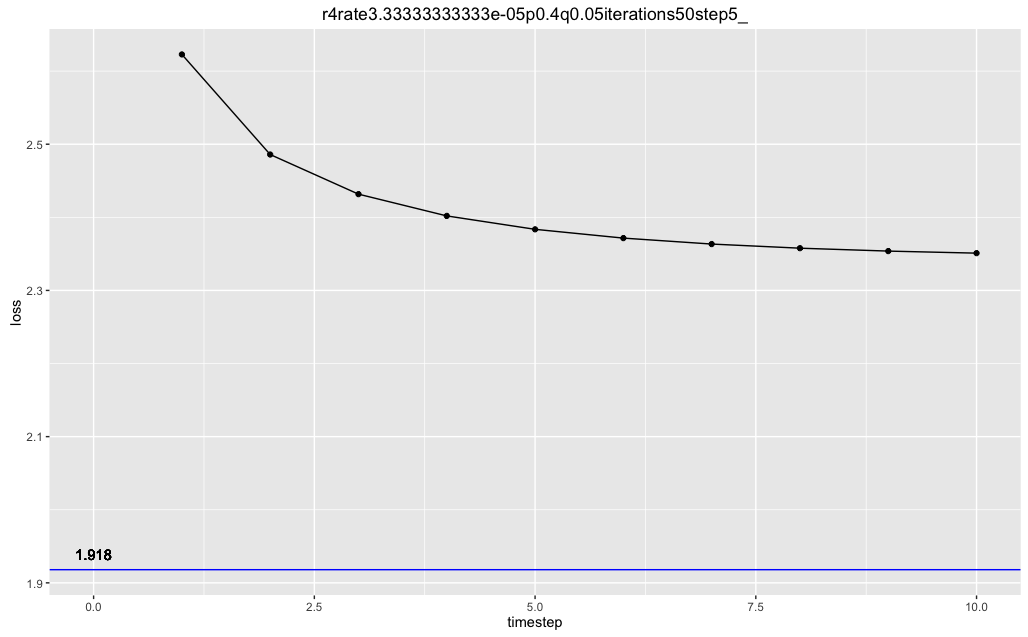
\includegraphics[width=0.8\textwidth]{50steps.png}
   \caption{$p=0.4, q=0.05$, 50 iterations}
  \label{fig:GNN_BH}
 \end{center}
\end{figure}

\begin{figure}
\begin{center}
  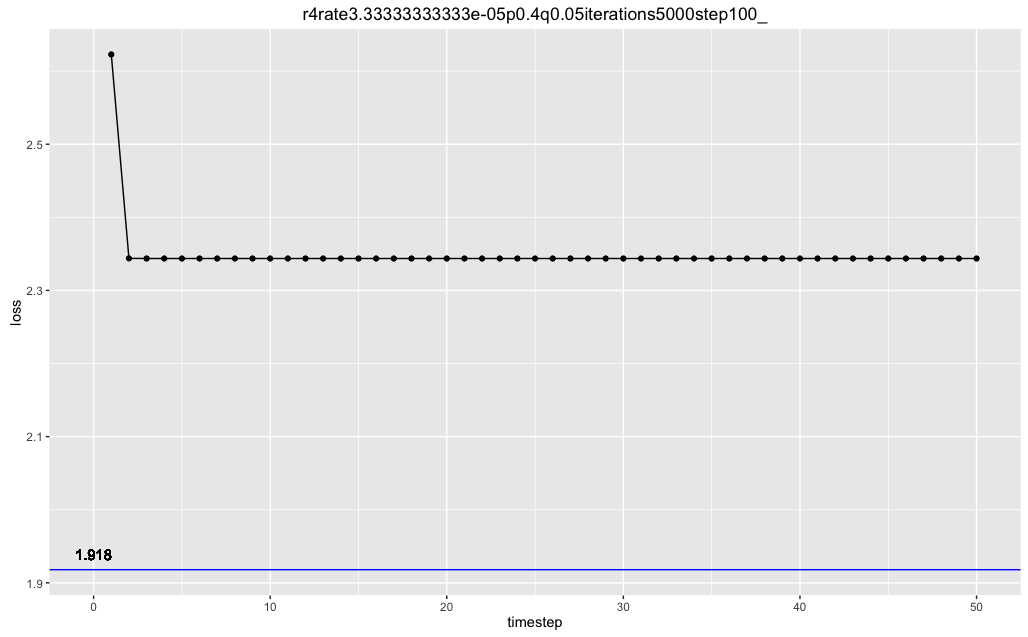
\includegraphics[width=0.8\textwidth]{500steps.png}
   \caption{$p=0.4, q=0.05$, 5000 iterations}
  \label{fig:GNN_BH_1}
 \end{center}
\end{figure}

\begin{figure}[H]
\begin{center}
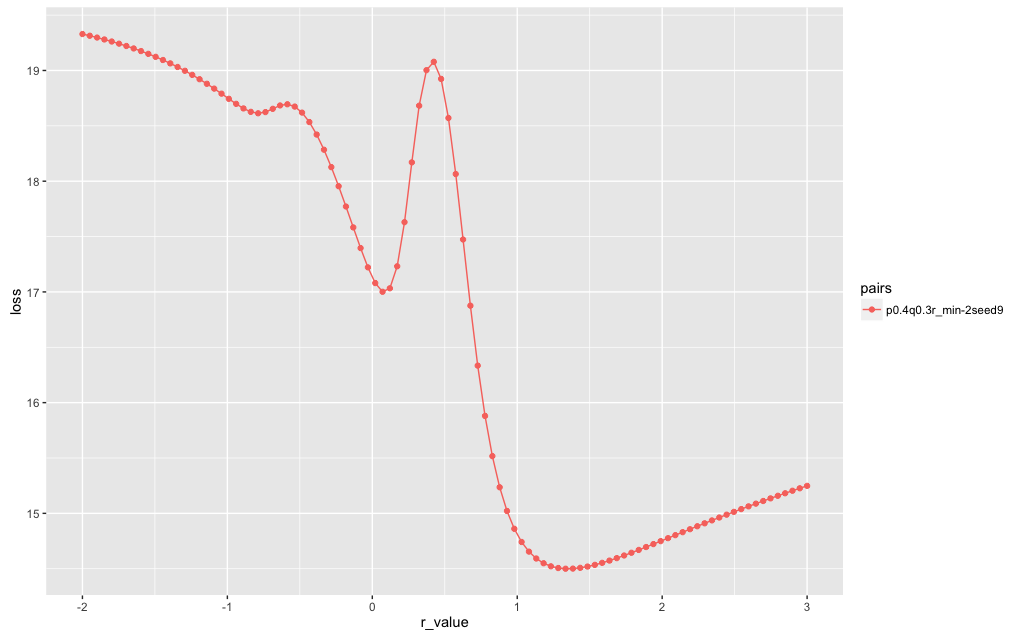
\includegraphics[scale=0.4]{loss_surface_1.png}
\caption{Bethe Hessian loss surface 1.}
 \end{center}
\end{figure}

\begin{figure}[H]
\begin{center}
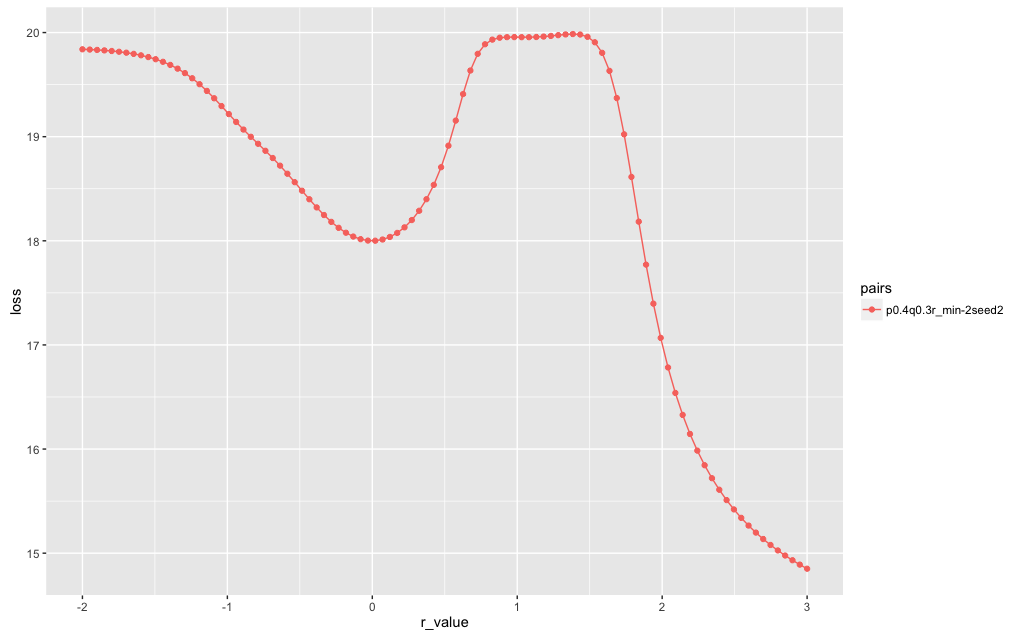
\includegraphics[scale=0.4]{loss_surface_2.png}
\caption{Bethe Hessian loss surface 2.}
 \end{center}
\end{figure}

\begin{figure}[H]
\begin{center}
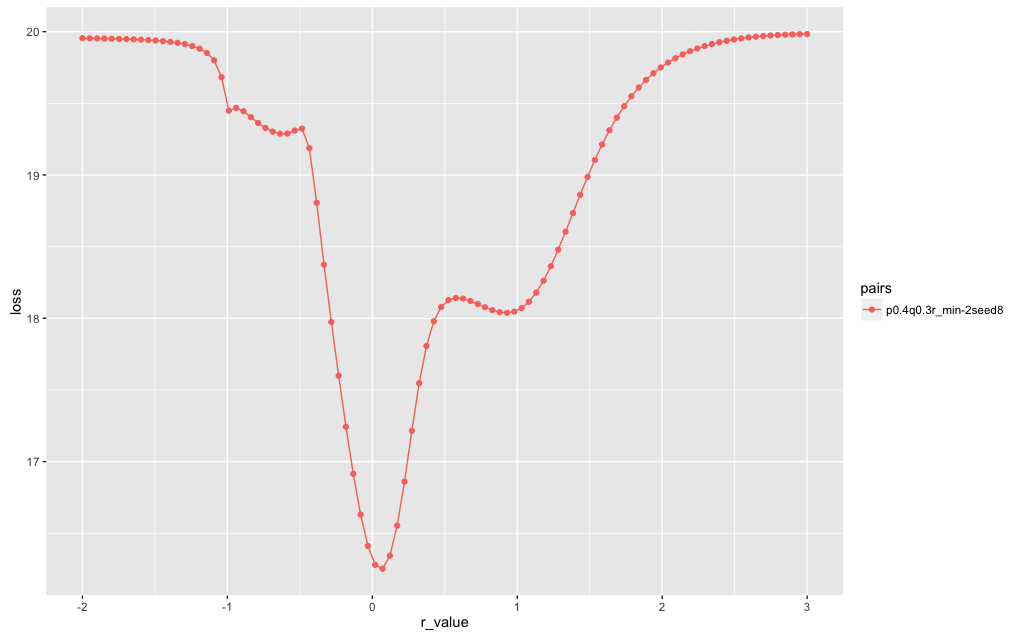
\includegraphics[scale=0.4]{loss_surface_3.png}
\caption{Bethe Hessian loss surface 3.}
 \end{center}
\end{figure}

\begin{figure}[H]
\begin{center}
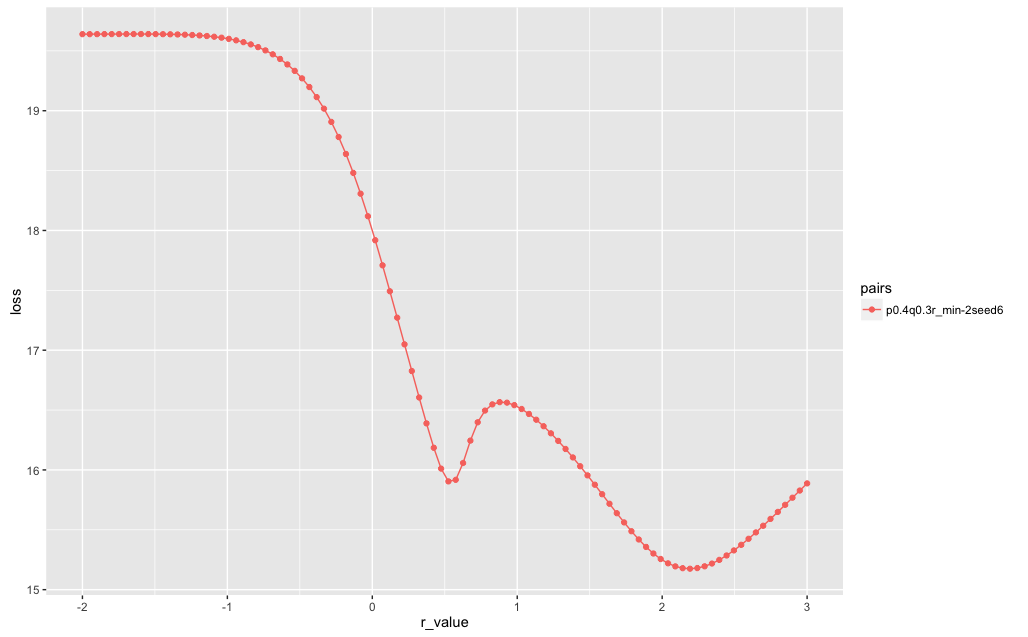
\includegraphics[scale=0.4]{loss_surface_4.png}
\caption{Bethe Hessian loss surface 4.}
 \end{center}
\end{figure}
 
Learning a one dimensional parameter $r$ is a proof of concept.  It forces an artificially hard bottleneck on our gradient optimization problem since the one dimensional loss surface is clearly non-convex and contains lots of non-optimal local optima. The optimization landscape is also highly varied depending on the instantiation of SBM.  What this section serves to confirm empirically is that the power method for a very specific matrix is within the expressive power of the GNN and that gradient descent can successfully find the scalar that best optimizes the spectral signal in that case. 

\newpage

\section{GNN Performance Near Information Theoretic Threshold}
\begin{figure}[H]
\begin{center}
  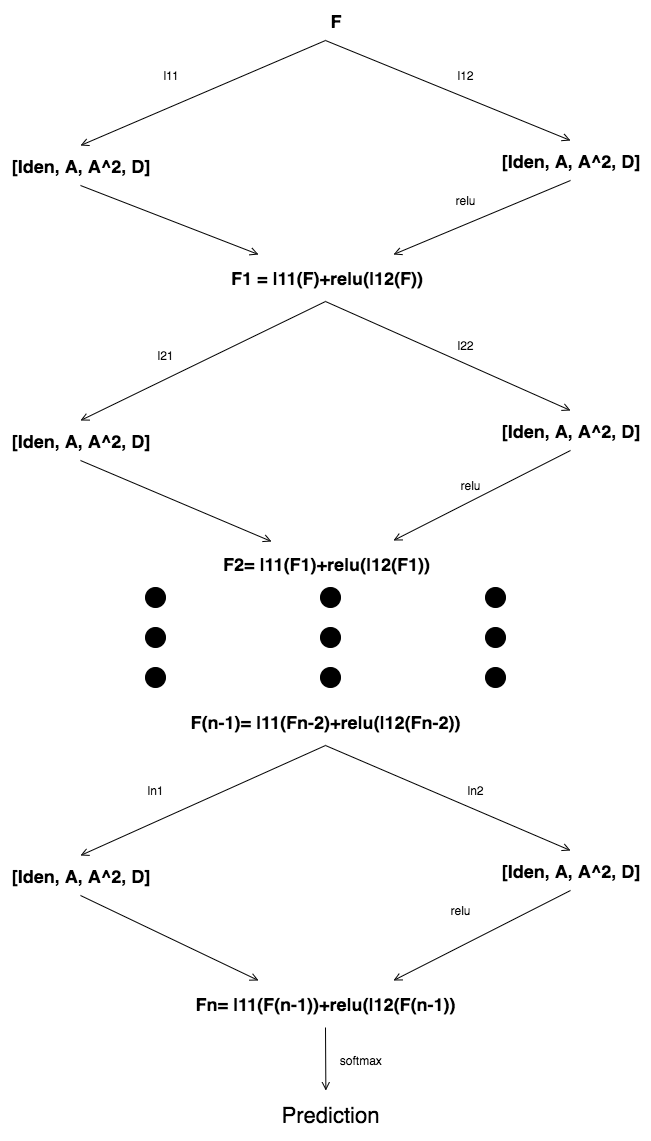
\includegraphics[scale=0.47]{GNN_SBM.png}
  \caption{Graph Neural Network architecture for information theoretic boundary for community detection.}
  \label{fig:GNN}
\end{center}
\end{figure}

For the main experiment, we consider a GNN with the structure shown in figure \ref{fig:GNN}.

In figure \ref{fig:GNN}, our input is $F\in \mathbb{R}^{n \times k}$ where $n$ is the number of nodes and $k$ is the dimension of the signal.  In a clustering problem, $k$ can be the number of communities we want to detect, where $\mathbb{R}^{n\times k}$ is a one-hot encoding of the clustering (an encoding where a categorical vector with $k$ categories is replaced with $k$ column vectors where each entry is 1 if it is in the category and 0 otherwise). At each layer, the input signal $F$ is transformed via a convolution applied to the following array of operators:  $[Iden, A, A^2, D]$.  $Iden$ is the identity matrix the size of the graph adjacency matrix.  $A$ is the graph adjacency matrix.  And $D$ is a matrix with the degree of each vertex on its diagonal (and zeros everywhere else). 

In the language of operators introduced in the previous section, each layer we have the following $$ F_1^{n+1} = \eta(Iden \cdot F^n, A \cdot F^n, A^2 \cdot F^n, D \cdot F^n)$$ and $$ F_2^{n+1} = Relu \circ \eta(Iden \cdot F^n, A \cdot F^n, A^2 \cdot F^n, D \cdot F^n)$$ and $$ F^{n+1} = F_1^{n+1}+F_2^{n+2}$$
where $\eta$ is a spatial convolution and $Relu(x) := max(0, x)$ (Relu applied to vectors would be Relu applied elementwise).  For our network applied to the SBM, we used 16 channels per layer, and 20 layers for a 1000 node graph. In the first layer each layer we apply a $k \times 4$ convolution to each of the 16 output channels.  The number of communities is given by $k$.  The final layer outputs to $k$ channels, to correspond to the $k$ dimensional one hot encoding of the community labels. We furthermore normalize and center after each layer for stability.  

The accuracy measure is given by the overlap. 
\begin{definition}The \textit{Overlap} between a true community label $g: V \rightarrow V$ where $g(u) := g_u$, and the predicted community label $\bar{g}:V \rightarrow V$ where $\bar{g}(u) := \bar{g_u}$, is given by
$$ \frac{\big(\frac{1}{n}\sum_u \delta_{g_u, \bar{g_u}} - \frac{1}{k}\big)}{(1-\frac{1}{k})}$$

where $\delta$ is the Kronecker delta function.  
\end{definition}

The clustering overlap performance of the GNN in the information theoretic threshold for the SBM in both assortative and dissortative regime are in graphs \ref{fig:ass}, \ref{fig:diss} and \ref{fig:k3}.  The regime is extremely sparse, where $n =1000$ and the average degree is $3$.  The x-axis is gives the difference in average degrees of the subgraph induced by nodes in the same community and between nodes in different communities: $c_{in} - c_{out}$.  Another way to interpret $c_in$ and $c_out$ is via $c_in/n = p$ and $c_out/n = q$.  The clustering problem becomes easier as $|c_in-c_out|$ grows.  

\begin{figure}[H]
\begin{center}
  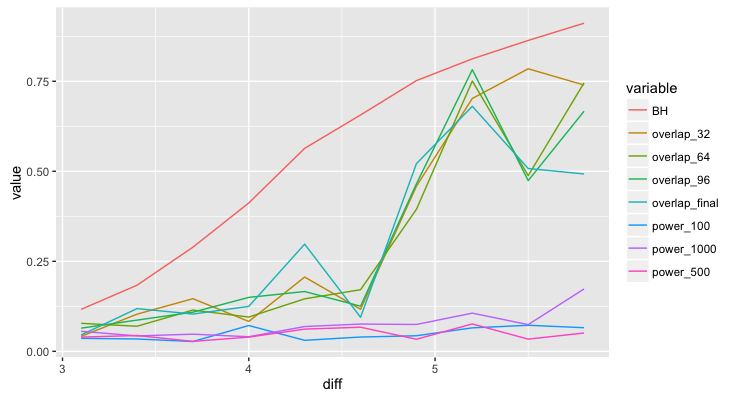
\includegraphics[scale=0.55]{asso.png}
  \caption{Performance of GNN against BH baseline for n=1000 at information theoretic threshold with assortative communities.}
  \label{fig:ass}
\end{center}
\end{figure}

\begin{figure}[H]
\begin{center}
  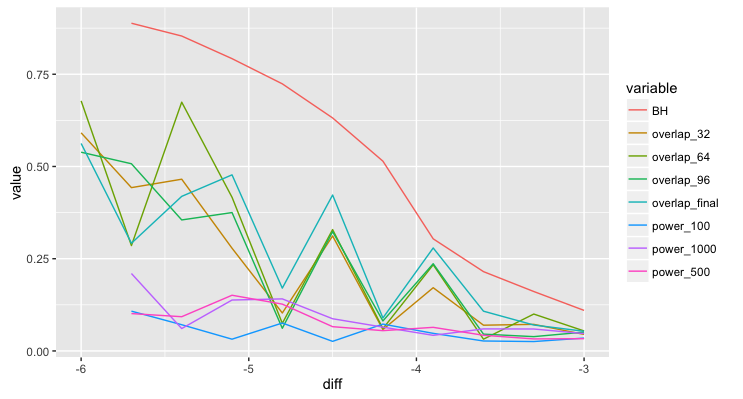
\includegraphics[scale=0.55]{diss.png}
  \caption{Performance of GNN against BH baseline for n=1000 at information theoretic threshold with dissortative communities.}
  \label{fig:diss}
\end{center}
\end{figure}

\begin{figure}[H]
\begin{center}
  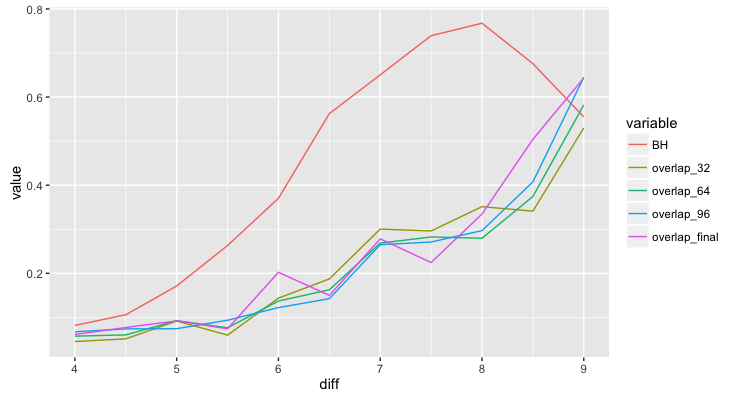
\includegraphics[scale=0.55]{k3.png}
  \caption{Performance of GNN against BH baseline for n=1000 at information theoretic threshold with 3 communities.}
  \label{fig:k3}
\end{center}
\end{figure}


\section{Future Directions}

We have shown the success of the graph neural network on even the most extreme cases of the SBM.  Current extensions of this work is being done by the author and Joan Bruna to apply to real datasets in the area of community detection in social networks, as well as more diverse problems that involve signals on graphs, including ranking, entity detection in databases and protein interaction detection. 

%\chapter{Future Directions}

We have shown the success of the graph neural network on even the most extreme cases of the SBM.  Current extensions of this work is being done by the current author to apply to real datasets in the area of community detection in social networks, as well as more diverse problems that involve of 

\appendix
\printbibliography


\end{document}
